% Sections/07-ThietKeHeThong.tex
% Chương 6 -- Thiết kế hệ thống
%=========================

\section{Thiết kế hệ thống}

Chương này chuyển các yêu cầu và quy trình đã phân tích ở chương trước thành thiết kế kỹ thuật cho hệ thống thương mại điện tử tích hợp AI Shopping Assistant. Nội dung tập trung vào cấu trúc thành phần, dữ liệu, giao tiếp, bảo mật và triển khai; các mô tả nghiệp vụ chi tiết không được lặp lại. Spring Boot Backend là cổng giao tiếp duy nhất của Frontend, còn MySQL là nguồn dữ liệu nghiệp vụ chính. AI Service hỗ trợ truy hồi và tư vấn nhưng không thay thế Backend trong việc xác nhận sản phẩm, giá, tồn kho và đơn hàng.

\subsection{Tổng quan thiết kế hệ thống}

\subsubsection{Phạm vi và ranh giới hệ thống}

Hệ thống được thiết kế cho hai nhóm tác nhân chính là khách hàng và quản trị viên. Khách hàng sử dụng các chức năng duyệt sản phẩm, tìm kiếm, trợ lý hội thoại, giỏ hàng và đặt hàng; quản trị viên vận hành catalog, tồn kho, đơn hàng, nội dung và quá trình đồng bộ chỉ mục AI. Trong phạm vi hiện tại, quy trình thanh toán được thiết kế cho phương thức thanh toán khi nhận hàng (COD); các cổng thanh toán trực tuyến không thuộc phạm vi triển khai.

Ranh giới hệ thống bao gồm Frontend, Spring Boot Backend, AI Service và các kho dữ liệu do ứng dụng quản lý. Trình duyệt chỉ gửi request đến Spring Boot Backend. Các nhà cung cấp mô hình, dịch vụ lưu trữ ảnh và hạ tầng triển khai được xem là hệ thống bên ngoài được truy cập thông qua adapter hoặc giao diện tích hợp. Cách xác định ranh giới này giúp tránh để client truy cập trực tiếp khóa mô hình, chỉ mục vector hoặc cơ sở dữ liệu nghiệp vụ.

\subsubsection{Mục tiêu và nguyên tắc thiết kế}

Thiết kế hệ thống hướng đến các mục tiêu sau:

\begin{itemize}
    \item Tách biệt nghiệp vụ thương mại điện tử khỏi các tác vụ AI để hai khối có thể phát triển và triển khai độc lập.
    \item Chỉ cho phép Frontend giao tiếp với Spring Boot Backend; AI Service được sử dụng như một dịch vụ nội bộ.
    \item Xem MySQL là nguồn dữ liệu chuẩn và Qdrant là chỉ mục phục vụ truy hồi có thể tái tạo.
    \item Hỗ trợ tìm kiếm bằng văn bản, hình ảnh, tìm kiếm kết hợp và hội thoại nhiều lượt.
    \item Lựa chọn LLM, embedding và reranker qua cấu hình thay vì gắn kiến trúc với một mô hình cụ thể.
    \item Cô lập lỗi AI khỏi giỏ hàng, đặt hàng, thanh toán và quản lý tồn kho.
\end{itemize}

Mỗi thành phần chỉ nắm giữ trách nhiệm thuộc phạm vi của mình. Mọi kết quả AI chứa mã sản phẩm phải được Backend đối chiếu lại với MySQL trước khi trả cho người dùng. Các tích hợp bên ngoài phải có timeout, kiểm tra lỗi và phương án dự phòng.

% \subsubsection{Các quyết định kiến trúc từ yêu cầu phi chức năng}

% Các quyết định thiết kế tổng quát được xây dựng từ nhóm yêu cầu phi chức năng ở Chương 5. Bảng~\ref{tab:overview-architecture-decisions} trình bày quan hệ giữa yêu cầu và giải pháp kiến trúc được lựa chọn.

% \begin{table}[H]
% \centering
% \caption{Ánh xạ yêu cầu phi chức năng với quyết định kiến trúc}
% \label{tab:overview-architecture-decisions}
% \begin{tabularx}{\linewidth}{@{}p{0.15\linewidth}p{0.23\linewidth}X@{}}
% \toprule
% \textbf{Yêu cầu} & \textbf{Thuộc tính} & \textbf{Quyết định thiết kế} \\
% \midrule
% NFR-01 & Hiệu năng & Giới hạn số kết quả, cấu hình timeout và tách các bước phân tích, embedding, retrieval, rerank để có thể đo thời gian từng bước. \\
% NFR-02 & Bảo mật & Sử dụng JWT, phân quyền theo vai trò, khóa API nội bộ và giới hạn truy cập MySQL, Qdrant trong mạng dịch vụ. \\
% NFR-03, NFR-04 & Khả dụng và tin cậy & Tách AI Service khỏi nghiệp vụ cốt lõi; MySQL giữ dữ liệu giao dịch và lỗi AI không làm mất hoặc sửa sai đơn hàng. \\
% NFR-05 & Bảo trì, mở rộng & Module hóa frontend, backend và AI Service; dùng adapter và biến môi trường để thay provider hoặc mô hình. \\
% NFR-06 & Tương thích & Frontend đáp ứng nhiều kích thước màn hình; các dịch vụ trao đổi dữ liệu JSON qua HTTP. \\
% NFR-07 & Khả năng quan sát & Cung cấp health check, metrics và log theo mã tương quan nhưng không ghi dữ liệu nhạy cảm. \\
% NFR-08 & Nhất quán & MySQL là nguồn chuẩn; Qdrant là chỉ mục có thể tái tạo; checkpoint hội thoại không thay thế dữ liệu giao dịch. \\
% NFR-09 & Tài nguyên AI & Ưu tiên provider được quản lý; embedding, reranker và phát hiện vật thể được bật, tắt hoặc thay thế qua cấu hình. \\
% \bottomrule
% \end{tabularx}
% \end{table}

\subsubsection{Kiến trúc tổng thể}

Hệ thống gồm Frontend React được phục vụ qua nginx, Spring Boot Backend, AI Service FastAPI, MySQL, Qdrant, kho checkpoint hội thoại, dịch vụ lưu trữ ảnh và các dịch vụ mô hình. Frontend cung cấp giao diện mua sắm và trợ lý; Spring Boot xử lý xác thực cùng toàn bộ nghiệp vụ; AI Service phân tích truy vấn, tạo embedding, truy hồi và điều phối hội thoại; MySQL lưu dữ liệu giao dịch; Qdrant lưu vector cùng metadata phục vụ tìm kiếm.

Trạng thái hội thoại được lưu qua checkpointer có Backend lựa chọn bằng cấu hình. SQLite phù hợp với môi trường đơn instance và kiểm thử; PostgreSQL hoặc Redis có thể được sử dụng khi cần chia sẻ trạng thái giữa nhiều instance. Ảnh sản phẩm được quản lý bằng URL và dịch vụ lưu trữ ảnh, trong khi health check, log và metrics cung cấp dữ liệu quan sát cho các thành phần vận hành. Các thành phần lưu trữ và giám sát này hỗ trợ hệ thống nhưng không nắm quyền quyết định đối với giao dịch thương mại điện tử.

\begin{figure}[H]
    \centering
    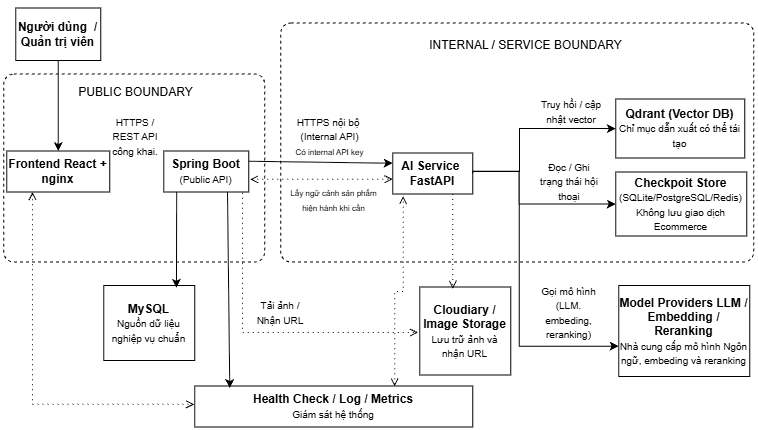
\includegraphics[width=0.98\textwidth]{Images/Thietkehethong/Kiến trúc tổng thể của hệ thống.drawio.drawio.png}
    \caption{Kiến trúc tổng thể của hệ thống}
    \label{fig:system-architecture}
\end{figure}

Hình~\ref{fig:system-architecture} phân chia hệ thống thành vùng truy cập công khai, vùng dịch vụ nội bộ và nhóm dịch vụ tích hợp bên ngoài. Người dùng và quản trị viên tương tác với Frontend React được phục vụ qua nginx. Frontend trao đổi với Spring Boot qua REST API công khai; Frontend không gọi trực tiếp AI Service hoặc các kho dữ liệu. Spring Boot vừa là cổng vào của hệ thống, vừa là thành phần điều phối nghiệp vụ và kiểm soát dữ liệu trả về client.

Trong vùng dịch vụ nội bộ, Spring Boot truy cập MySQL để xử lý dữ liệu nghiệp vụ và gọi AI Service FastAPI qua API nội bộ có khóa xác thực. AI Service truy vấn hoặc cập nhật vector trong Qdrant, đồng thời đọc và ghi checkpoint phục vụ hội thoại nhiều lượt. Khi cần phân tích truy vấn, sinh embedding, rerank hoặc tạo câu trả lời, AI Service gọi nhà cung cấp mô hình thông qua adapter tương ứng. Chiều gọi ngược từ AI Service về Spring Boot chỉ được sử dụng để lấy ngữ cảnh sản phẩm hiện hành khi cần; AI Service không truy cập trực tiếp MySQL.

Cloudinary hoặc dịch vụ lưu trữ ảnh tiếp nhận tệp từ Backend và trả URL để lưu cùng dữ liệu catalog. AI Service có thể tải ảnh thông qua URL cho quá trình lập chỉ mục hoặc tìm kiếm ảnh. Các thành phần Frontend, Spring Boot và AI Service đồng thời phát sinh health check, log và metrics để theo dõi trạng thái, độ trễ và lỗi. Cách bố trí này tạo ranh giới rõ giữa dữ liệu giao dịch, dữ liệu dẫn xuất và dịch vụ AI, qua đó hạn chế sự cố ở một thành phần lan sang toàn bộ hệ thống.

\subsubsection{Quyền sở hữu và vòng đời dữ liệu}

Mỗi kho dữ liệu được sử dụng cho một mục đích riêng. Việc xác định nguồn dữ liệu chuẩn giúp hệ thống xử lý đúng khi thông tin trong các kho tạm thời chưa đồng bộ.

\begin{table}[H]
\centering
\caption{Vai trò và quyền sở hữu dữ liệu của các kho lưu trữ}
\label{tab:overview-data-ownership}
\begin{tabularx}{\linewidth}{|p{0.20\linewidth}|p{0.41\linewidth}|X|}
\hline
\textbf{Kho dữ liệu} & \textbf{Vai trò} & \textbf{Nguyên tắc sử dụng} \\ \hline
MySQL & Lưu tài khoản, catalog, giá, tồn kho, giỏ hàng, đơn hàng và thanh toán. & Là nguồn dữ liệu nghiệp vụ chuẩn và được bảo vệ bằng giao dịch. \\ \hline
Qdrant & Lưu vector văn bản, vector hình ảnh và metadata truy hồi. & Là chỉ mục dẫn xuất; có thể tái tạo từ dữ liệu sản phẩm và không quyết định dữ liệu hiển thị cuối cùng. \\ \hline
Kho checkpoint & Lưu trạng thái workflow, tóm tắt, ràng buộc và lựa chọn theo phiên hội thoại. & Có thể dùng SQLite, PostgreSQL hoặc Redis theo môi trường; không lưu giao dịch thương mại điện tử. \\ \hline
Dịch vụ lưu trữ ảnh & Lưu tệp ảnh và cung cấp URL cho catalog hoặc truy vấn ảnh. & Backend kiểm tra tệp và chỉ lưu URL cần thiết trong dữ liệu sản phẩm. \\ \hline
Log và metrics & Lưu thông tin lỗi, latency và trạng thái vận hành. & Chỉ phục vụ quan sát, không chứa token, bí mật hoặc nội dung nhạy cảm không cần thiết. \\ \hline
\end{tabularx}
\end{table}

\subsubsection{Luồng xử lý tổng quát}

Hệ thống có ba luồng xử lý tổng quát. Thứ nhất, luồng thương mại điện tử đi từ Frontend đến Spring Boot, thực hiện kiểm tra quyền và nghiệp vụ, truy cập MySQL rồi trả response cho Frontend. Luồng này không phụ thuộc vào Qdrant hoặc nhà cung cấp mô hình.

Thứ hai, luồng AI trực tuyến bắt đầu khi Frontend gửi truy vấn văn bản, ảnh hoặc hội thoại đến Spring Boot. Backend xác thực và chuyển dữ liệu cần thiết sang AI Service. AI Service đọc checkpoint khi có phiên hội thoại, phân tích truy vấn, tạo embedding, truy hồi Qdrant và có thể gọi mô hình để tạo phản hồi. Danh sách mã sản phẩm được trả về Spring Boot để đối chiếu lại với MySQL trước khi gửi kết quả cuối cùng đến Frontend.

Thứ ba, luồng đồng bộ chỉ mục được kích hoạt bởi quản trị viên hoặc tác vụ hệ thống. Spring Boot đọc sản phẩm từ MySQL, chuẩn hóa dữ liệu và gửi theo batch đến AI Service. AI Service tạo embedding rồi thêm, cập nhật hoặc xóa vector trong Qdrant. Lỗi đồng bộ được ghi nhận để thử lại nhưng không hoàn tác dữ liệu nghiệp vụ đã lưu thành công trong MySQL.

Ba luồng trên sử dụng chung nguyên tắc: Spring Boot kiểm soát ranh giới công khai, dữ liệu giao dịch chỉ được ghi tại MySQL, còn các thành phần AI có thể suy giảm độc lập. Vì vậy, khi AI Service, Qdrant hoặc nhà cung cấp mô hình tạm thời không khả dụng, người dùng vẫn có thể duyệt catalog, quản lý giỏ hàng và thực hiện các nghiệp vụ thương mại điện tử còn lại.

\subsection{Thiết kế kiến trúc}

\subsubsection{Kiến trúc phía máy khách}

Frontend được xây dựng dưới dạng ứng dụng trang đơn bằng React. Mã nguồn được chia thành các nhóm \texttt{Pages}, \texttt{Layouts}, \texttt{components}, \texttt{Route}, \texttt{redux}, \texttt{api} và các tiện ích dùng chung. Cách tổ chức này tách màn hình nghiệp vụ khỏi thành phần trình bày có thể tái sử dụng, đồng thời tập trung việc định tuyến, quản lý trạng thái và giao tiếp HTTP vào các mô-đun riêng.

Các trang và layout chịu trách nhiệm ghép thành phần giao diện theo từng luồng sử dụng. React Router ánh xạ URL đến trang tương ứng; \texttt{PrivateRoute} kiểm tra trạng thái đăng nhập trước khi hiển thị các màn hình được bảo vệ. Việc kiểm tra này chỉ phục vụ trải nghiệm phía máy khách, còn quyền truy cập thực sự vẫn được Spring Security xác minh tại Backend, vì trạng thái trên trình duyệt có thể bị thay đổi bởi người dùng.

Trạng thái dùng chung được quản lý bằng Redux. Một số dữ liệu phục vụ tính liên tục của giao diện được lưu cục bộ, chẳng hạn trạng thái đăng nhập và giỏ hàng trong \texttt{localStorage}, mã phiên trợ lý trong \texttt{sessionStorage}. Đây không phải nguồn dữ liệu nghiệp vụ chuẩn: giá bán, tồn kho, trạng thái đơn hàng và quyền người dùng luôn phải được đối chiếu lại qua API trước khi thực hiện thao tác có ảnh hưởng đến hệ thống.

Lớp \texttt{api} tập trung các lời gọi HTTP thông qua một Axios instance dùng chung. Interceptor gắn access token vào request và xử lý trạng thái hết phiên theo một quy tắc thống nhất. Các chức năng tìm kiếm văn bản, tìm kiếm ảnh, tìm kiếm lai và trợ lý hội thoại được khai báo tại \texttt{aiApi}, nhưng tất cả đều gọi endpoint của Spring Boot. Vì vậy Frontend không giữ khóa truy cập AI, không kết nối trực tiếp AI Service, MySQL hoặc Qdrant và không tự quyết định kết quả nghiệp vụ.

\begin{table}[H]
    \centering
    \caption{Các nhóm thành phần chính của Frontend}
    \label{tab:frontend-components}
    \begin{tabularx}{\textwidth}{|p{0.23\textwidth}|X|}
        \hline
        \textbf{Nhóm thành phần} & \textbf{Trách nhiệm} \\
        \hline
        Trang và bố cục & Tổ chức màn hình theo luồng nghiệp vụ và xác định cấu trúc hiển thị chung. \\
        \hline
        Thành phần giao diện & Đóng gói các phần tử có thể tái sử dụng, tiếp nhận dữ liệu qua thuộc tính và phát sinh sự kiện người dùng. \\
        \hline
        Định tuyến & Ánh xạ URL đến màn hình, điều hướng và kiểm tra điều kiện hiển thị các tuyến riêng tư. \\
        \hline
        Redux và lưu trữ cục bộ & Quản lý trạng thái dùng chung và duy trì một số trạng thái giao diện qua lần tải lại trang. \\
        \hline
        API và tiện ích & Chuẩn hóa URL, header xác thực, cách gửi request, xử lý lỗi và chuyển đổi dữ liệu phục vụ giao diện. \\
        \hline
    \end{tabularx}
\end{table}

\subsubsection{Kiến trúc Spring Boot Backend}

Backend được tổ chức theo kiến trúc phân lớp để tách giao tiếp HTTP, quy tắc nghiệp vụ, truy cập dữ liệu và tích hợp bên ngoài. Mỗi lớp chỉ phụ thuộc vào giao diện của lớp kế tiếp, nhờ đó thay đổi ở cơ sở dữ liệu hoặc AI Service không buộc Frontend thay đổi theo.

\begin{figure}[H]
    \centering
    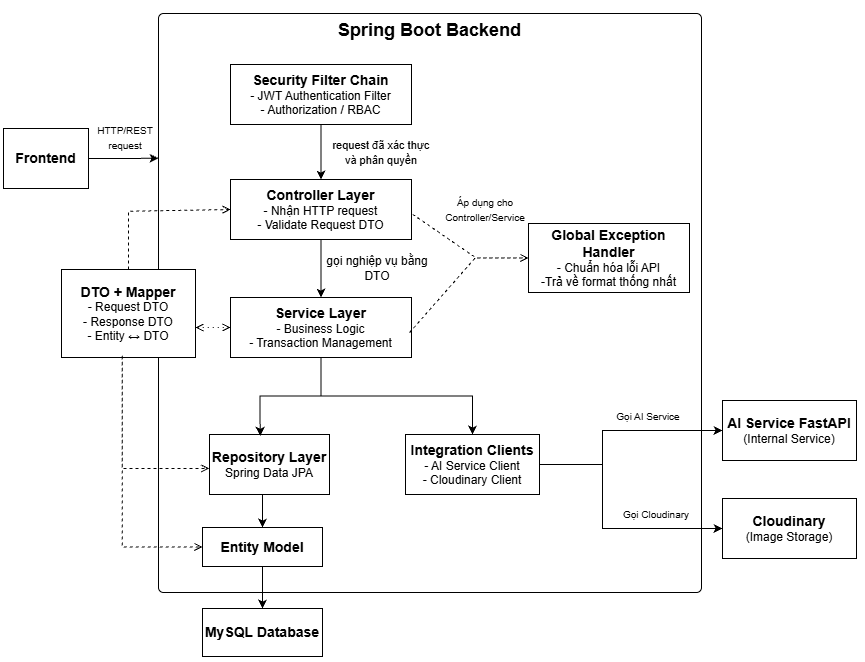
\includegraphics[width=0.98\textwidth]{Images/Thietkehethong/Kiến trúc phân lớp của Spring Boot Backend.drawio.png}
    \caption{Kiến trúc phân lớp của Spring Boot Backend}
    \label{fig:backend-layers}
\end{figure}

Như trình bày tại Hình~\ref{fig:backend-layers}, request từ Frontend trước hết đi qua Security Filter Chain. JWT Authentication Filter đọc và kiểm tra access token, sau đó thiết lập thông tin xác thực cho request. Cấu hình phân quyền quyết định endpoint nào được truy cập công khai, endpoint nào yêu cầu đăng nhập và nhóm \texttt{/admin} nào yêu cầu vai trò quản trị. Khi xác thực hoặc phân quyền thất bại, \texttt{AuthenticationEntryPoint} và \texttt{AccessDeniedHandler} lần lượt chuẩn hóa phản hồi HTTP 401 và 403.

Sau lớp bảo mật, Controller tiếp nhận request, ánh xạ tham số và kiểm tra Request DTO. Controller không chứa quy tắc nghiệp vụ phức tạp mà chuyển dữ liệu hợp lệ xuống Service. Service là lớp trung tâm thực hiện nghiệp vụ, kiểm tra các ràng buộc liên miền và xác định phạm vi giao dịch. Những thao tác cần cập nhật nhất quán nhiều bảng, chẳng hạn tạo đơn hàng, giữ tồn kho hoặc ghi nhận thanh toán, được quản lý transaction tại lớp này.

Repository sử dụng Spring Data JPA để thao tác với MySQL thông qua các Entity ánh xạ bảng. MySQL nằm ngoài tiến trình Spring Boot và là nguồn dữ liệu nghiệp vụ chuẩn. DTO được dùng tại ranh giới API, còn Mapper chuyển đổi giữa DTO và Entity; do đó cấu trúc bảng không bị để lộ trực tiếp cho Frontend và thay đổi response không nhất thiết làm thay đổi mô hình lưu trữ.

Các kết nối ra ngoài được đóng gói trong Integration Clients. AI Service Client chuyển các yêu cầu tìm kiếm, hội thoại và đồng bộ chỉ mục đến AI Service FastAPI; Cloudinary Client thực hiện tải ảnh và nhận URL lưu trữ. Cách đóng gói này tập trung cấu hình URL, xác thực, timeout và xử lý lỗi của từng dịch vụ. Ngoại lệ phát sinh từ Controller hoặc Service được Global Exception Handler chuyển thành cấu trúc lỗi API thống nhất, trong khi chi tiết kỹ thuật chỉ được ghi trong log của Backend.

\subsubsection{Kiến trúc AI Service}

AI Service được triển khai bằng FastAPI và tổ chức theo hướng mô-đun. Tầng \texttt{api/routes} công bố các endpoint tìm kiếm, trợ lý, đồng bộ chỉ mục, kiểm tra trạng thái và số liệu vận hành; các schema định nghĩa cấu trúc request và response tại ranh giới dịch vụ. Route chỉ xác thực dữ liệu đầu vào và chuyển yêu cầu đến lớp dịch vụ, không chứa chi tiết của mô hình AI hay kho vector.

Lớp dịch vụ gồm các mô-đun \texttt{search}, \texttt{embeddings}, \texttt{cropping}, \texttt{query\_understanding}, \texttt{reranking}, \texttt{assistant} và \texttt{indexing}. Mỗi mô-đun đảm nhiệm một bước độc lập trong chuỗi xử lý. Các adapter thuộc tầng \texttt{infrastructure} đóng gói kết nối đến Qdrant, Spring Boot và nhà cung cấp mô hình. Nhờ phụ thuộc vào giao diện chung thay vì một hiện thực cố định, hệ thống có thể lựa chọn nhà cung cấp LLM, embedding và reranking bằng cấu hình môi trường mà không phải thay đổi route nghiệp vụ.

Với yêu cầu tìm kiếm, dữ liệu đầu vào được chuẩn hóa và phân tích để nhận diện từ khóa hoặc bộ lọc có cấu trúc. Mô-đun embedding chuyển văn bản hay ảnh thành vector; Search Service truy vấn Qdrant để lấy tập ứng viên và có thể gọi reranker để sắp xếp lại. Kết quả trả về chỉ gồm định danh sản phẩm, điểm số và thông tin giải thích cần thiết. Spring Boot dùng các định danh này để lấy dữ liệu hiện hành từ MySQL, loại bỏ sản phẩm không còn hợp lệ và tạo response cuối cùng cho Frontend.

Đối với tìm kiếm ảnh, mô-đun cropping có thể sử dụng toàn bộ ảnh, vùng do người dùng chọn hoặc vùng đối tượng được YOLO phát hiện. YOLO là thành phần tùy chọn; khi bị tắt hoặc không tìm thấy đối tượng phù hợp, chuỗi xử lý vẫn tiếp tục bằng ảnh gốc. Thiết kế suy giảm này tránh biến mô-đun phát hiện đối tượng thành điểm lỗi bắt buộc của chức năng tìm kiếm ảnh.

Trợ lý hội thoại được tổ chức thành workflow có trạng thái. Workflow tiếp nhận câu hỏi và ngữ cảnh phiên, phân loại nhu cầu, gọi công cụ tìm kiếm hoặc API ngữ cảnh của Spring Boot khi cần, sau đó mới tạo câu trả lời. Checkpoint lưu trạng thái hội thoại theo phiên và có thể được cấu hình trên SQLite, PostgreSQL hoặc Redis. Dữ liệu checkpoint hỗ trợ tiếp tục hội thoại nhưng không thay thế hồ sơ người dùng hay dữ liệu giao dịch trong MySQL.

Luồng indexing nhận dữ liệu sản phẩm đã được Spring Boot chuẩn hóa, tạo các biểu diễn vector cần thiết và ghi hoặc cập nhật điểm tương ứng trong Qdrant. Vì Qdrant chỉ là chỉ mục dẫn xuất, toàn bộ chỉ mục có thể được xây dựng lại từ dữ liệu chuẩn khi thay đổi mô hình embedding, cấu trúc payload hoặc khi cần phục hồi. Các endpoint health, readiness và metrics cung cấp khả năng quan sát trạng thái phụ thuộc, thời gian xử lý và lỗi của các chuỗi AI.

\begin{table}[H]
    \centering
    \caption{Trách nhiệm các mô-đun chính của AI Service}
    \label{tab:ai-service-components}
    \begin{tabularx}{\textwidth}{|p{0.25\textwidth}|X|}
        \hline
        \textbf{Mô-đun} & \textbf{Trách nhiệm} \\
        \hline
        API và schema & Kiểm tra dữ liệu, công bố hợp đồng HTTP và chuyển yêu cầu đến dịch vụ phù hợp. \\
        \hline
        Query understanding & Chuẩn hóa truy vấn và trích xuất ý định, từ khóa hoặc bộ lọc tìm kiếm. \\
        \hline
        Embedding, cropping và reranking & Tiền xử lý dữ liệu đa phương thức, tạo vector và cải thiện thứ tự tập ứng viên. \\
        \hline
        Search Service & Điều phối chuỗi truy vấn Qdrant và trả về định danh cùng điểm số ứng viên. \\
        \hline
        Assistant workflow & Quản lý luồng hội thoại, sử dụng công cụ và lưu checkpoint của phiên. \\
        \hline
        Indexing Service & Chuyển dữ liệu sản phẩm chuẩn hóa thành payload và vector có thể tái tạo trong Qdrant. \\
        \hline
        Infrastructure adapters & Cô lập kết nối Qdrant, Spring Boot, kho checkpoint và các nhà cung cấp mô hình. \\
        \hline
    \end{tabularx}
\end{table}

\subsubsection{Giao tiếp và phân chia trách nhiệm}

Các thành phần giao tiếp theo nguyên tắc một cổng công khai. Frontend chỉ gọi API của Spring Boot bằng HTTPS và JSON; access token được gửi trong header xác thực đối với endpoint yêu cầu đăng nhập. Spring Boot xác thực người dùng, kiểm tra quyền, thực hiện nghiệp vụ và chỉ chuyển sang AI Service phần dữ liệu tối thiểu cần cho tác vụ AI. Trình duyệt vì vậy không cần biết địa chỉ nội bộ hoặc thông tin xác thực của AI Service.

Spring Boot gọi AI Service qua HTTP nội bộ với khóa API giữa dịch vụ, timeout hữu hạn và cấu trúc lỗi được chuẩn hóa. Các thao tác có thể được gọi lại, đặc biệt là cập nhật chỉ mục, cần mang định danh ổn định để tránh tạo bản ghi vector trùng lặp. Khi AI Service trả về danh sách ứng viên, Backend lấy lại dữ liệu từ MySQL theo định danh, bảo toàn thứ tự xếp hạng nếu còn hợp lệ, rồi áp dụng các điều kiện nghiệp vụ trước khi phản hồi cho Frontend.

Theo chiều ngược lại, AI Service chỉ được gọi một tập API ngữ cảnh giới hạn của Spring Boot, chẳng hạn thông tin sản phẩm cần cho trợ lý. AI Service không dùng tài khoản cơ sở dữ liệu và không truy cập trực tiếp MySQL. Ranh giới này giúp các quy tắc phân quyền, lọc dữ liệu nhạy cảm và kiểm soát phiên bản dữ liệu vẫn tập trung tại Backend.

\begin{table}[H]
    \centering
    \caption{Hợp đồng giao tiếp giữa các thành phần}
    \label{tab:service-communication-contracts}
    \begin{tabularx}{\textwidth}{|p{0.20\textwidth}|p{0.21\textwidth}|X|}
        \hline
        \textbf{Kênh giao tiếp} & \textbf{Cơ chế bảo vệ} & \textbf{Trách nhiệm và cách xử lý lỗi} \\
        \hline
        Frontend $\rightarrow$ Spring Boot & HTTPS, JWT và kiểm tra quyền tại Backend & Spring Boot xác thực request, trả mã lỗi API thống nhất; Frontend chỉ hiển thị trạng thái và yêu cầu người dùng thao tác lại khi cần. \\
        \hline
        Spring Boot $\rightarrow$ AI Service & Mạng nội bộ, khóa API dịch vụ và timeout & Backend gửi dữ liệu tối thiểu, kiểm tra response và chuyển lỗi phụ thuộc thành phản hồi phù hợp; nghiệp vụ thương mại điện tử không phụ thuộc AI vẫn tiếp tục hoạt động. \\
        \hline
        AI Service $\rightarrow$ Spring Boot & API ngữ cảnh giới hạn và xác thực dịch vụ & AI Service chỉ đọc ngữ cảnh được cấp phép, không truy cập MySQL; khi thiếu ngữ cảnh, workflow trả kết quả suy giảm thay vì tự suy đoán dữ liệu giao dịch. \\
        \hline
    \end{tabularx}
\end{table}

\subsection{Thiết kế dữ liệu}

\subsubsection{Mô hình dữ liệu tổng quan}

Dữ liệu MySQL được phân chia thành các miền nghiệp vụ nhằm giới hạn trách nhiệm
của từng nhóm bảng và thuận lợi cho việc bảo trì. Sơ đồ tổng quan thể hiện các
bảng, khóa chính, khóa ngoại quan trọng và quan hệ giữa các miền; thuộc tính chi
tiết của từng bảng được trình bày trong các sơ đồ thành phần ở phần tiếp theo.

\begin{figure}[H]
    \centering
    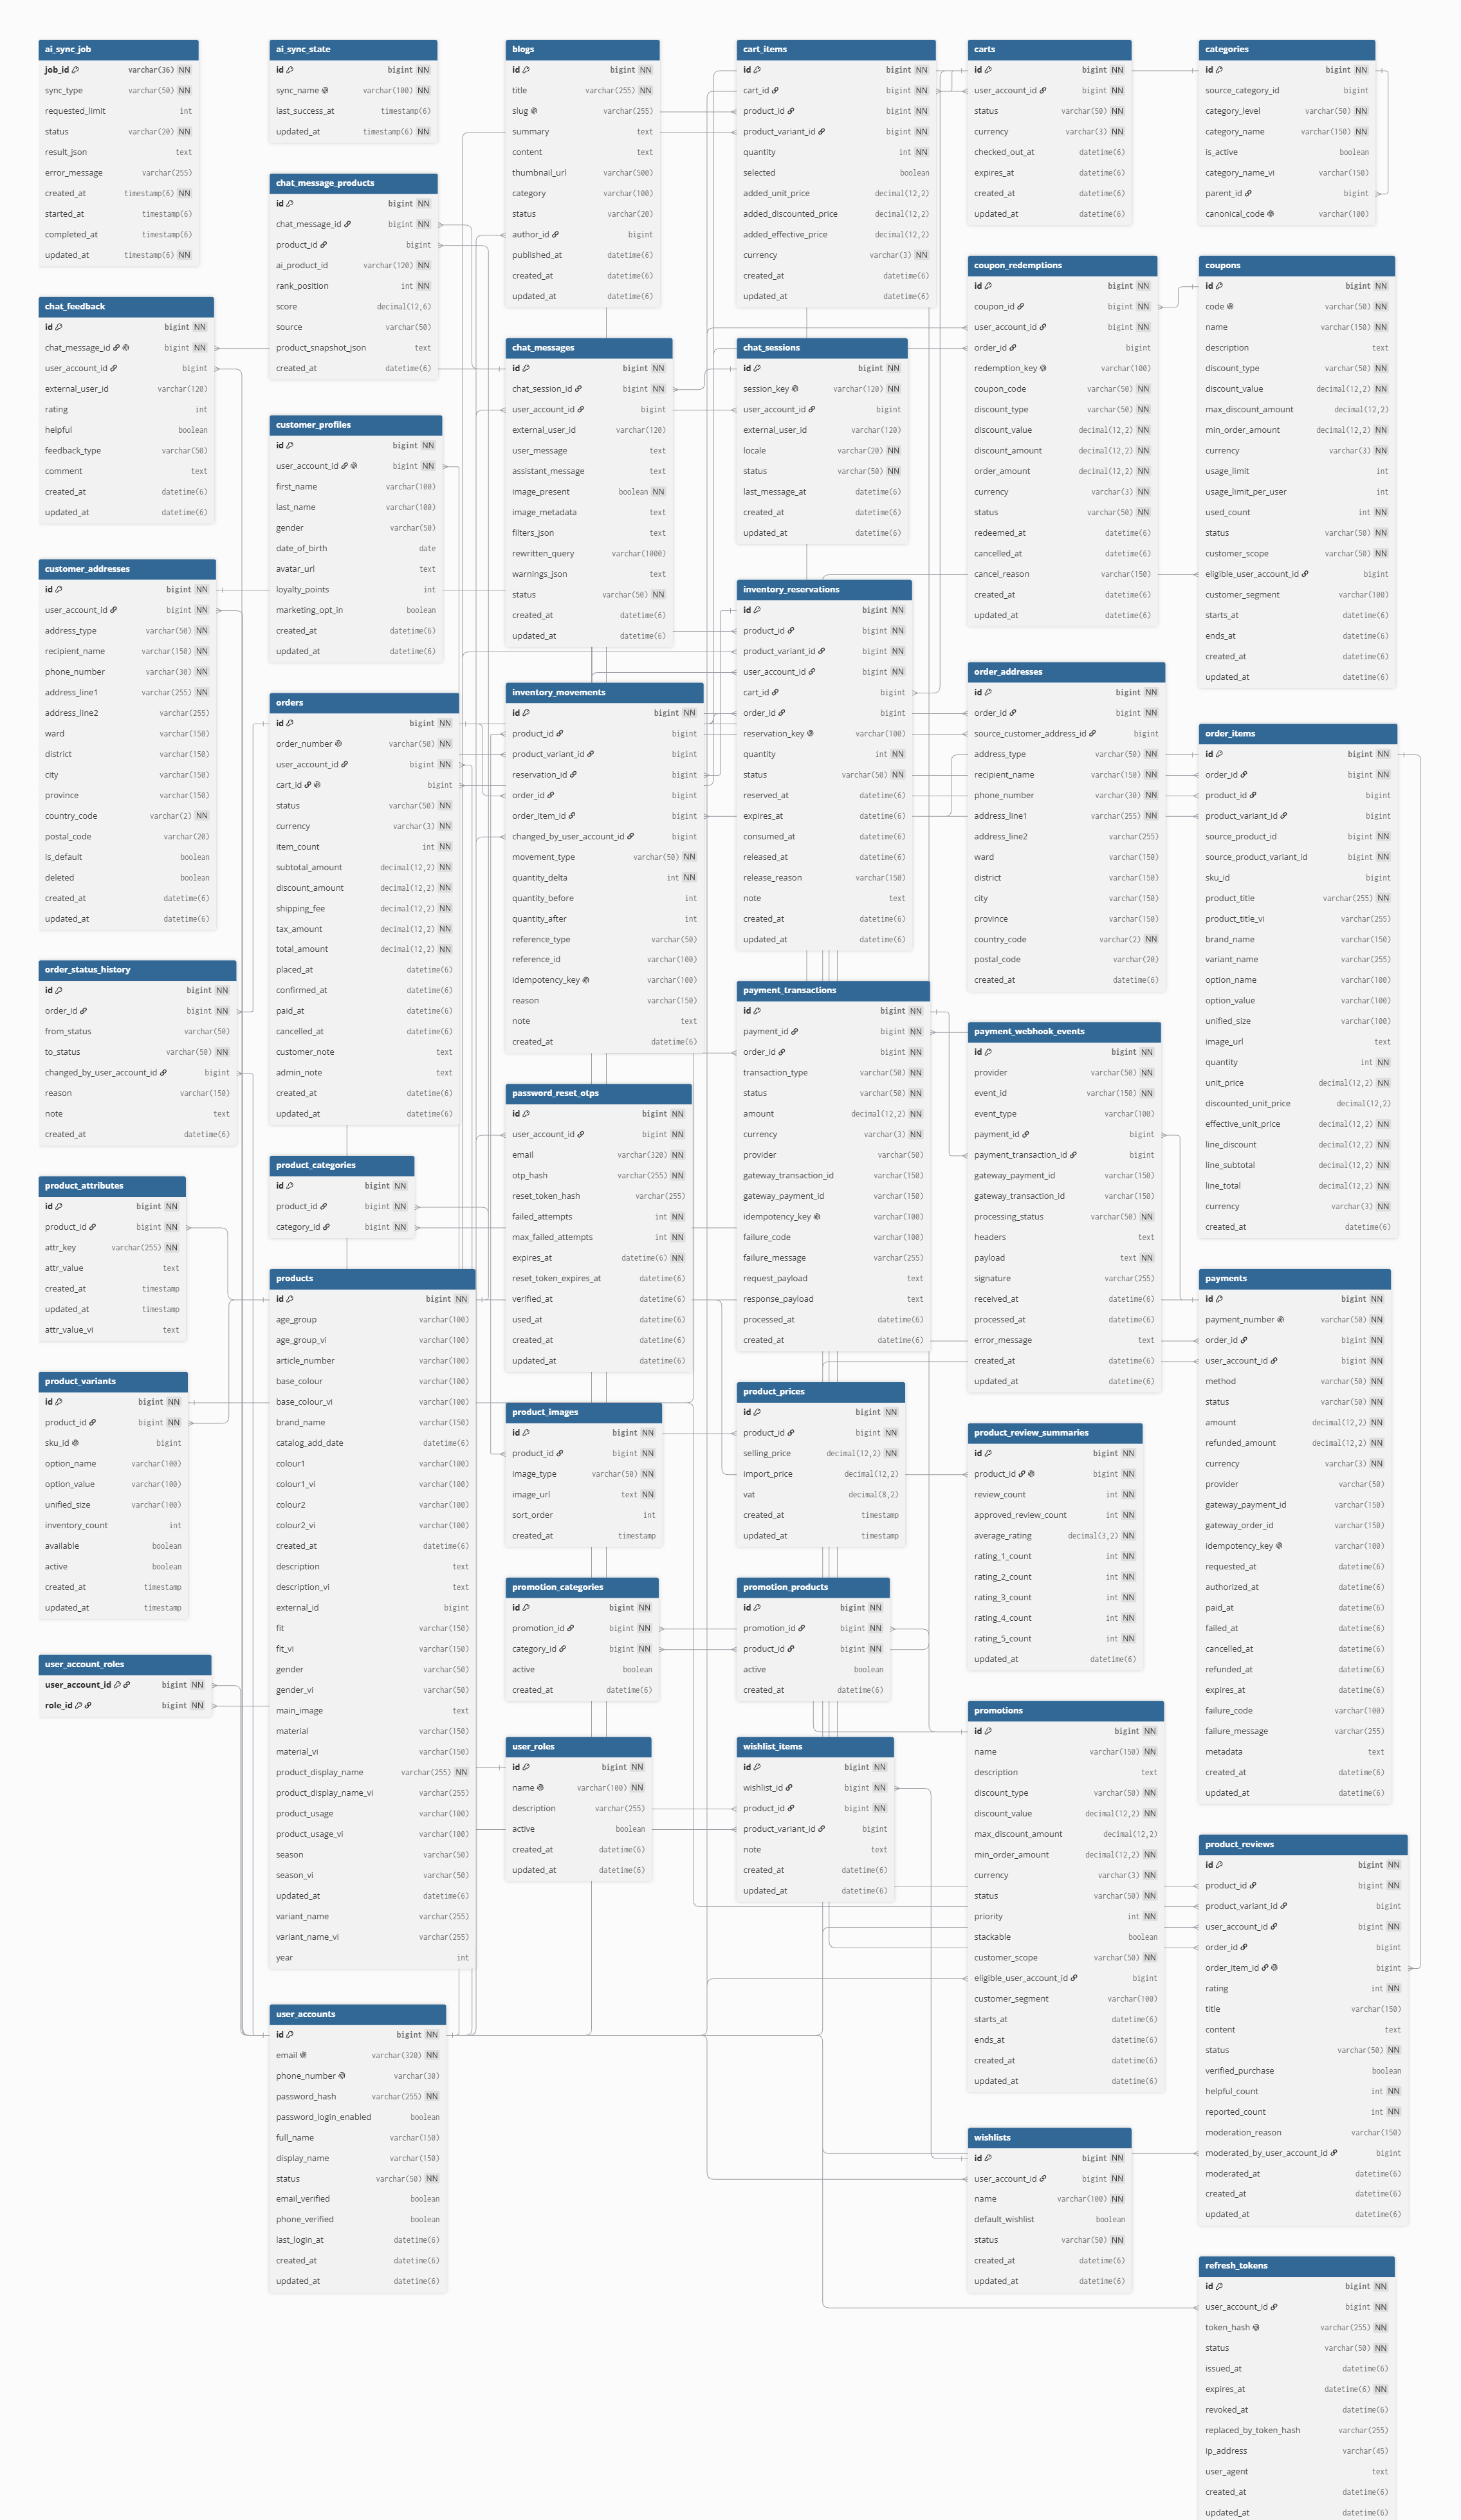
\includegraphics[
        width=\textwidth,
        height=0.82\textheight,
        keepaspectratio
    ]{Images/Thietkehethong/sơ đồ tổng quan toàn bộ cơ sở dữ liệu.png}
    \caption{Sơ đồ tổng quan toàn bộ cơ sở dữ liệu}
    \label{fig:database-overview}
\end{figure}

\subsubsection{Nhóm dữ liệu người dùng và phân quyền}

Nhóm này quản lý thông tin đăng nhập, hồ sơ, địa chỉ, vai trò và vòng đời thông
tin xác thực của người dùng. Quan hệ nhiều--nhiều giữa tài khoản và vai trò được
cài đặt qua bảng liên kết; refresh token và mã OTP khôi phục mật khẩu được lưu
riêng để có thể thu hồi, giới hạn thời gian sử dụng và truy vết độc lập.

\begin{figure}[H]
    \centering
    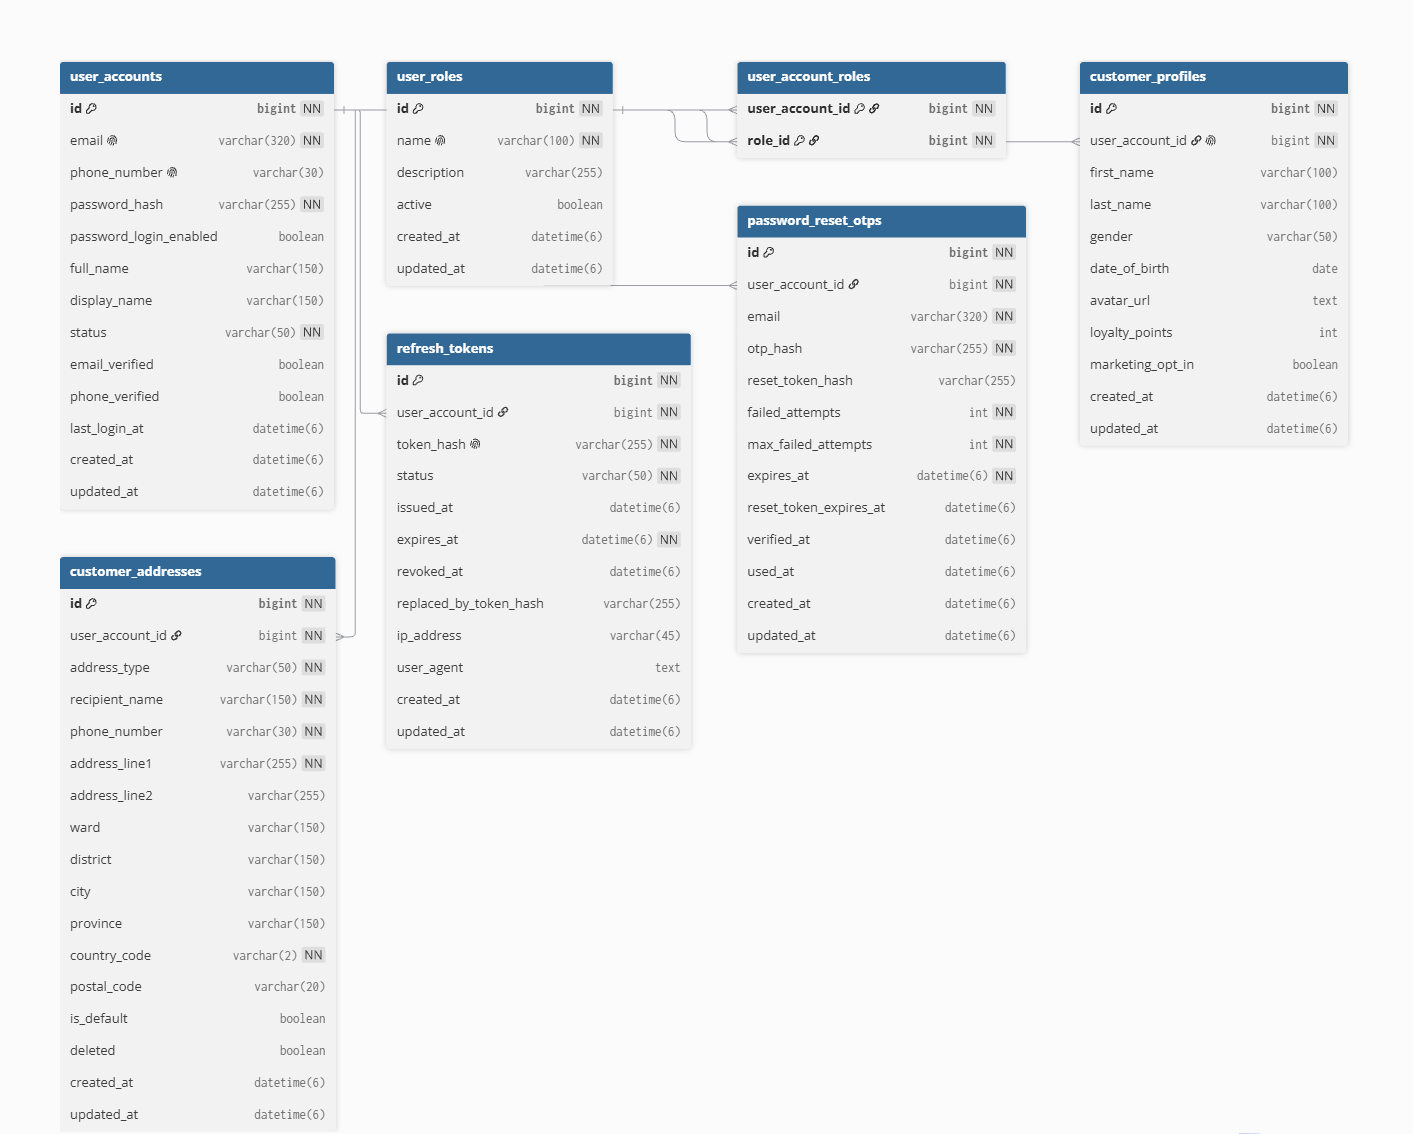
\includegraphics[
        width=\textwidth,
        height=0.72\textheight,
        keepaspectratio
    ]{Images/Thietkehethong/Người dùng và phân quyền.png}
    \caption{Sơ đồ dữ liệu người dùng và phân quyền}
    \label{fig:database-user-authorization}
\end{figure}

Trong Hình~\ref{fig:database-user-authorization}, \texttt{user\_accounts} là
thực thể trung tâm. Mỗi tài khoản có tối đa một hồ sơ khách hàng và có thể sở hữu
nhiều địa chỉ, refresh token hoặc yêu cầu đặt lại mật khẩu. Quan hệ giữa tài
khoản và vai trò được chuẩn hóa qua \texttt{user\_account\_roles}, cho phép mở
rộng tập vai trò mà không phải thay đổi cấu trúc tài khoản.

Bảng~\ref{tab:data-summary-user-authorization} tóm tắt chức năng của các bảng trong nhóm. Chỉ các bảng cốt lõi, đại diện trực tiếp cho luồng nghiệp vụ chính, được mô tả chi tiết trường dữ liệu.

\begin{longtable}{|>{\RaggedRight\arraybackslash}p{0.34\textwidth}|>{\RaggedRight\arraybackslash}p{0.56\textwidth}|}
    \caption{Các bảng thuộc nhóm người dùng và phân quyền}
    \label{tab:data-summary-user-authorization} \\
    \hline
    \textbf{Tên bảng} & \textbf{Chức năng} \\
    \hline
    \endfirsthead
    \multicolumn{2}{c}{\tablename\ \thetable\ (tiếp theo)} \\
    \hline
    \textbf{Tên bảng} & \textbf{Chức năng} \\
    \hline
    \endhead
    \texttt{user\_accounts} & Tài khoản người dùng. \\
    \hline
    \texttt{user\_roles} & Vai trò người dùng. \\
    \hline
    \texttt{user\_account\_roles} & Gán vai trò cho tài khoản. \\
    \hline
    \texttt{customer\_profiles} & Hồ sơ khách hàng. \\
    \hline
    \texttt{customer\_addresses} & Địa chỉ khách hàng. \\
    \hline
    \texttt{refresh\_tokens} & Refresh token. \\
    \hline
    \texttt{password\_reset\_otps} & Mã OTP đặt lại mật khẩu. \\
    \hline
\end{longtable}

\paragraph{Các bảng cốt lõi.}

\begin{longtable}{|>{\RaggedRight\arraybackslash}p{0.25\textwidth}|>{\RaggedRight\arraybackslash}p{0.20\textwidth}|>{\RaggedRight\arraybackslash}p{0.45\textwidth}|}
    \caption{Mô tả chi tiết bảng \texttt{user\_accounts} (Tài khoản người dùng)}
    \label{tab:data-dictionary-user-accounts} \\
    \hline
    \textbf{Tên trường} & \textbf{Kiểu dữ liệu} & \textbf{Mô tả} \\
    \hline
    \endfirsthead
    \multicolumn{3}{c}{\tablename\ \thetable\ (tiếp theo)} \\
    \hline
    \textbf{Tên trường} & \textbf{Kiểu dữ liệu} & \textbf{Mô tả} \\
    \hline
    \endhead
    \texttt{\seqsplit{id}} & \texttt{bigint} & Khóa chính tự tăng. \\
        \hline
        \texttt{\seqsplit{email}} & \texttt{varchar(320)} & Địa chỉ thư điện tử; bắt buộc; duy nhất. \\
        \hline
        \texttt{\seqsplit{phone\_number}} & \texttt{varchar(30)} & Số điện thoại; duy nhất. \\
        \hline
        \texttt{\seqsplit{password\_hash}} & \texttt{varchar(255)} & Giá trị băm của mật khẩu; bắt buộc. \\
        \hline
        \texttt{\seqsplit{password\_login\_enabled}} & \texttt{boolean} & Cho biết tài khoản có cho phép đăng nhập bằng mật khẩu. \\
        \hline
        \texttt{\seqsplit{full\_name}} & \texttt{varchar(150)} & Họ và tên đầy đủ. \\
        \hline
        \texttt{\seqsplit{display\_name}} & \texttt{varchar(150)} & Tên hiển thị. \\
        \hline
        \texttt{\seqsplit{status}} & \texttt{varchar(50)} & Trạng thái hiện tại; bắt buộc. \\
        \hline
        \texttt{\seqsplit{email\_verified}} & \texttt{boolean} & Cho biết email đã được xác minh. \\
        \hline
        \texttt{\seqsplit{phone\_verified}} & \texttt{boolean} & Cho biết số điện thoại đã được xác minh. \\
        \hline
        \texttt{\seqsplit{last\_login\_at}} & \texttt{datetime(6)} & Thời điểm đăng nhập gần nhất. \\
        \hline
        \texttt{\seqsplit{created\_at}} & \texttt{datetime(6)} & Thời điểm tạo bản ghi. \\
        \hline
        \texttt{\seqsplit{updated\_at}} & \texttt{datetime(6)} & Thời điểm cập nhật gần nhất. \\
        \hline
\end{longtable}

\begin{longtable}{|>{\RaggedRight\arraybackslash}p{0.25\textwidth}|>{\RaggedRight\arraybackslash}p{0.20\textwidth}|>{\RaggedRight\arraybackslash}p{0.45\textwidth}|}
    \caption{Mô tả chi tiết bảng \texttt{user\_roles} (Vai trò người dùng)}
    \label{tab:data-dictionary-user-roles} \\
    \hline
    \textbf{Tên trường} & \textbf{Kiểu dữ liệu} & \textbf{Mô tả} \\
    \hline
    \endfirsthead
    \multicolumn{3}{c}{\tablename\ \thetable\ (tiếp theo)} \\
    \hline
    \textbf{Tên trường} & \textbf{Kiểu dữ liệu} & \textbf{Mô tả} \\
    \hline
    \endhead
    \texttt{\seqsplit{id}} & \texttt{bigint} & Khóa chính tự tăng. \\
        \hline
        \texttt{\seqsplit{name}} & \texttt{varchar(100)} & Tên; bắt buộc; duy nhất. \\
        \hline
        \texttt{\seqsplit{description}} & \texttt{varchar(255)} & Nội dung mô tả. \\
        \hline
        \texttt{\seqsplit{active}} & \texttt{boolean} & Cho biết bản ghi đang hoạt động. \\
        \hline
        \texttt{\seqsplit{created\_at}} & \texttt{datetime(6)} & Thời điểm tạo bản ghi. \\
        \hline
        \texttt{\seqsplit{updated\_at}} & \texttt{datetime(6)} & Thời điểm cập nhật gần nhất. \\
        \hline
\end{longtable}



\subsubsection{Nhóm dữ liệu danh mục và sản phẩm}

Nhóm danh mục và sản phẩm lưu dữ liệu mô tả hàng hóa, cấu trúc danh mục, biến
thể, thuộc tính, hình ảnh và giá bán. Bảng \texttt{products} đóng vai trò trung
tâm; các quan hệ thành phần được tách thành bảng riêng để một sản phẩm có thể có
nhiều danh mục, biến thể, thuộc tính và hình ảnh mà không lặp dữ liệu nền.

\begin{figure}[H]
    \centering
    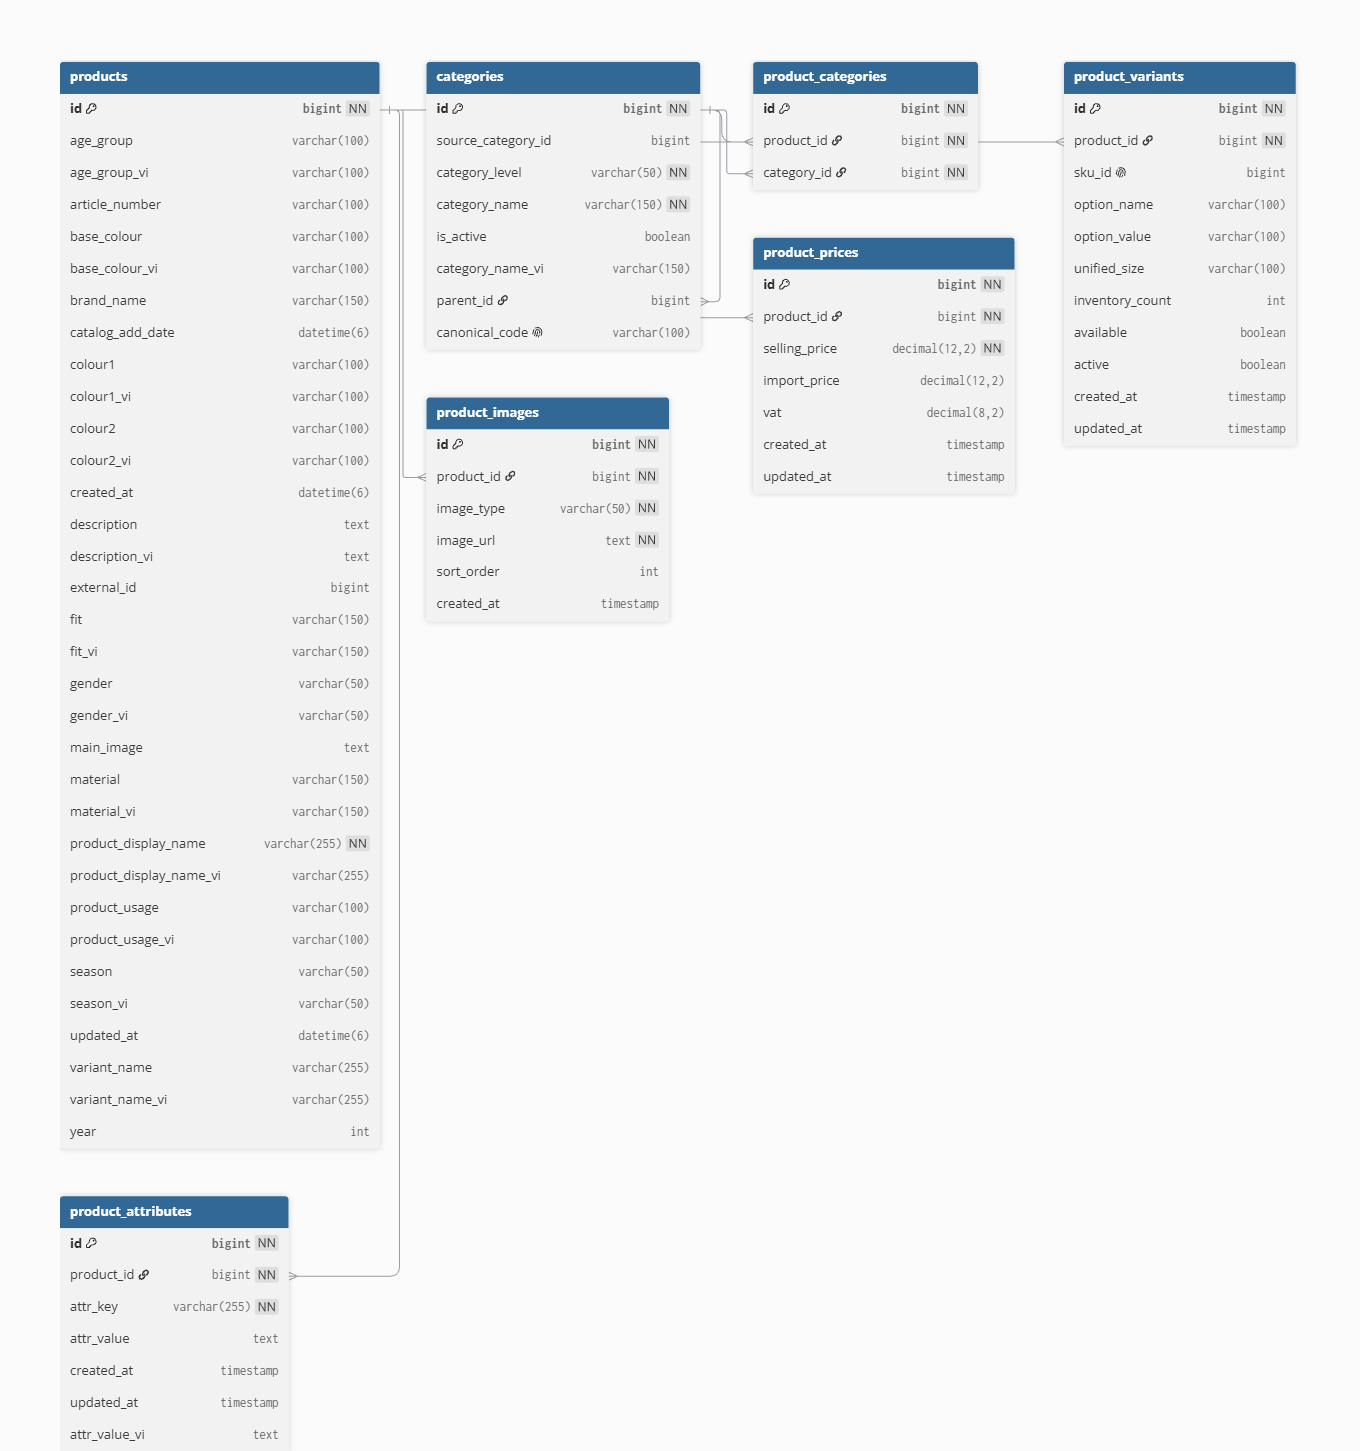
\includegraphics[
        width=\textwidth,
        height=0.72\textheight,
        keepaspectratio
    ]{Images/Thietkehethong/Danh mục và sản phẩm.png}
    \caption{Sơ đồ dữ liệu danh mục và sản phẩm}
    \label{fig:database-catalog-product}
\end{figure}

Hình~\ref{fig:database-catalog-product} cho thấy một sản phẩm có thể thuộc nhiều
danh mục thông qua bảng liên kết sản phẩm--danh mục; bản thân danh mục có quan hệ
cha--con để biểu diễn cấu trúc phân cấp. Biến thể, thuộc tính, hình ảnh và giá
được tách khỏi \texttt{products}, nhờ đó các tập dữ liệu có số lượng thay đổi
độc lập và không làm lặp lại thông tin mô tả chung của sản phẩm.

Bảng~\ref{tab:data-summary-catalog-product} tóm tắt chức năng của các bảng trong nhóm. Chỉ các bảng cốt lõi, đại diện trực tiếp cho luồng nghiệp vụ chính, được mô tả chi tiết trường dữ liệu.

\begin{longtable}{|>{\RaggedRight\arraybackslash}p{0.34\textwidth}|>{\RaggedRight\arraybackslash}p{0.56\textwidth}|}
    \caption{Các bảng thuộc nhóm danh mục và sản phẩm}
    \label{tab:data-summary-catalog-product} \\
    \hline
    \textbf{Tên bảng} & \textbf{Chức năng} \\
    \hline
    \endfirsthead
    \multicolumn{2}{c}{\tablename\ \thetable\ (tiếp theo)} \\
    \hline
    \textbf{Tên bảng} & \textbf{Chức năng} \\
    \hline
    \endhead
    \texttt{products} & Sản phẩm. \\
    \hline
    \texttt{categories} & Danh mục sản phẩm. \\
    \hline
    \texttt{product\_categories} & Liên kết sản phẩm--danh mục. \\
    \hline
    \texttt{product\_variants} & Biến thể sản phẩm. \\
    \hline
    \texttt{product\_attributes} & Thuộc tính sản phẩm. \\
    \hline
    \texttt{product\_images} & Hình ảnh sản phẩm. \\
    \hline
    \texttt{product\_prices} & Giá sản phẩm. \\
    \hline
\end{longtable}

\paragraph{Các bảng cốt lõi.}

\begin{longtable}{|>{\RaggedRight\arraybackslash}p{0.25\textwidth}|>{\RaggedRight\arraybackslash}p{0.20\textwidth}|>{\RaggedRight\arraybackslash}p{0.45\textwidth}|}
    \caption{Mô tả chi tiết bảng \texttt{products} (Sản phẩm)}
    \label{tab:data-dictionary-products} \\
    \hline
    \textbf{Tên trường} & \textbf{Kiểu dữ liệu} & \textbf{Mô tả} \\
    \hline
    \endfirsthead
    \multicolumn{3}{c}{\tablename\ \thetable\ (tiếp theo)} \\
    \hline
    \textbf{Tên trường} & \textbf{Kiểu dữ liệu} & \textbf{Mô tả} \\
    \hline
    \endhead
    \texttt{\seqsplit{id}} & \texttt{bigint} & Khóa chính. \\
        \hline
        \texttt{\seqsplit{age\_group}} & \texttt{varchar(100)} & Nhóm tuổi của sản phẩm. \\
        \hline
        \texttt{\seqsplit{age\_group\_vi}} & \texttt{varchar(100)} & Nhóm tuổi bằng tiếng Việt. \\
        \hline
        \texttt{\seqsplit{article\_number}} & \texttt{varchar(100)} & Mã bài hàng của sản phẩm. \\
        \hline
        \texttt{\seqsplit{base\_colour}} & \texttt{varchar(100)} & Màu cơ bản. \\
        \hline
        \texttt{\seqsplit{base\_colour\_vi}} & \texttt{varchar(100)} & Màu cơ bản bằng tiếng Việt. \\
        \hline
        \texttt{\seqsplit{brand\_name}} & \texttt{varchar(150)} & Tên thương hiệu. \\
        \hline
        \texttt{\seqsplit{catalog\_add\_date}} & \texttt{datetime(6)} & Thời điểm sản phẩm được thêm vào danh mục. \\
        \hline
        \texttt{\seqsplit{colour1}} & \texttt{varchar(100)} & Màu thứ nhất. \\
        \hline
        \texttt{\seqsplit{colour1\_vi}} & \texttt{varchar(100)} & Màu thứ nhất bằng tiếng Việt. \\
        \hline
        \texttt{\seqsplit{colour2}} & \texttt{varchar(100)} & Màu thứ hai. \\
        \hline
        \texttt{\seqsplit{colour2\_vi}} & \texttt{varchar(100)} & Màu thứ hai bằng tiếng Việt. \\
        \hline
        \texttt{\seqsplit{created\_at}} & \texttt{datetime(6)} & Thời điểm tạo bản ghi. \\
        \hline
        \texttt{\seqsplit{description}} & \texttt{text} & Nội dung mô tả. \\
        \hline
        \texttt{\seqsplit{description\_vi}} & \texttt{text} & Mô tả bằng tiếng Việt. \\
        \hline
        \texttt{\seqsplit{external\_id}} & \texttt{bigint} & Định danh sản phẩm tại nguồn ngoài. \\
        \hline
        \texttt{\seqsplit{fit}} & \texttt{varchar(150)} & Kiểu dáng. \\
        \hline
        \texttt{\seqsplit{fit\_vi}} & \texttt{varchar(150)} & Kiểu dáng bằng tiếng Việt. \\
        \hline
        \texttt{\seqsplit{gender}} & \texttt{varchar(50)} & Giới tính. \\
        \hline
        \texttt{\seqsplit{gender\_vi}} & \texttt{varchar(50)} & Giới tính bằng tiếng Việt. \\
        \hline
        \texttt{\seqsplit{main\_image}} & \texttt{text} & Đường dẫn ảnh đại diện chính. \\
        \hline
        \texttt{\seqsplit{material}} & \texttt{varchar(150)} & Chất liệu. \\
        \hline
        \texttt{\seqsplit{material\_vi}} & \texttt{varchar(150)} & Chất liệu bằng tiếng Việt. \\
        \hline
        \texttt{\seqsplit{product\_display\_name}} & \texttt{varchar(255)} & Tên hiển thị của sản phẩm; bắt buộc. \\
        \hline
        \texttt{\seqsplit{product\_display\_name\_vi}} & \texttt{varchar(255)} & Tên hiển thị bằng tiếng Việt. \\
        \hline
        \texttt{\seqsplit{product\_usage}} & \texttt{varchar(100)} & Mục đích sử dụng. \\
        \hline
        \texttt{\seqsplit{product\_usage\_vi}} & \texttt{varchar(100)} & Mục đích sử dụng bằng tiếng Việt. \\
        \hline
        \texttt{\seqsplit{season}} & \texttt{varchar(50)} & Mùa sử dụng. \\
        \hline
        \texttt{\seqsplit{season\_vi}} & \texttt{varchar(50)} & Mùa sử dụng bằng tiếng Việt. \\
        \hline
        \texttt{\seqsplit{updated\_at}} & \texttt{datetime(6)} & Thời điểm cập nhật gần nhất. \\
        \hline
        \texttt{\seqsplit{variant\_name}} & \texttt{varchar(255)} & Tên biến thể. \\
        \hline
        \texttt{\seqsplit{variant\_name\_vi}} & \texttt{varchar(255)} & Tên biến thể bằng tiếng Việt. \\
        \hline
        \texttt{\seqsplit{year}} & \texttt{int} & Năm của mẫu sản phẩm. \\
        \hline
\end{longtable}

\begin{longtable}{|>{\RaggedRight\arraybackslash}p{0.25\textwidth}|>{\RaggedRight\arraybackslash}p{0.20\textwidth}|>{\RaggedRight\arraybackslash}p{0.45\textwidth}|}
    \caption{Mô tả chi tiết bảng \texttt{categories} (Danh mục sản phẩm)}
    \label{tab:data-dictionary-categories} \\
    \hline
    \textbf{Tên trường} & \textbf{Kiểu dữ liệu} & \textbf{Mô tả} \\
    \hline
    \endfirsthead
    \multicolumn{3}{c}{\tablename\ \thetable\ (tiếp theo)} \\
    \hline
    \textbf{Tên trường} & \textbf{Kiểu dữ liệu} & \textbf{Mô tả} \\
    \hline
    \endhead
    \texttt{\seqsplit{id}} & \texttt{bigint} & Khóa chính tự tăng. \\
        \hline
        \texttt{\seqsplit{source\_category\_id}} & \texttt{bigint} & Định danh danh mục tại nguồn dữ liệu ngoài. \\
        \hline
        \texttt{\seqsplit{category\_level}} & \texttt{varchar(50)} & Cấp của danh mục; bắt buộc. \\
        \hline
        \texttt{\seqsplit{category\_name}} & \texttt{varchar(150)} & Tên danh mục; bắt buộc. \\
        \hline
        \texttt{\seqsplit{is\_active}} & \texttt{boolean} & Cho biết danh mục đang được kích hoạt và có thể sử dụng. \\
        \hline
        \texttt{\seqsplit{category\_name\_vi}} & \texttt{varchar(150)} & Tên danh mục bằng tiếng Việt. \\
        \hline
        \texttt{\seqsplit{parent\_id}} & \texttt{bigint} & Khóa ngoại tham chiếu \texttt{categories.id}. \\
        \hline
        \texttt{\seqsplit{canonical\_code}} & \texttt{varchar(100)} & Mã chuẩn duy nhất của danh mục; duy nhất. \\
        \hline
\end{longtable}

\begin{longtable}{|>{\RaggedRight\arraybackslash}p{0.25\textwidth}|>{\RaggedRight\arraybackslash}p{0.20\textwidth}|>{\RaggedRight\arraybackslash}p{0.45\textwidth}|}
    \caption{Mô tả chi tiết bảng \texttt{product\_images} (Hình ảnh sản phẩm)}
    \label{tab:data-dictionary-product-images} \\
    \hline
    \textbf{Tên trường} & \textbf{Kiểu dữ liệu} & \textbf{Mô tả} \\
    \hline
    \endfirsthead
    \multicolumn{3}{c}{\tablename\ \thetable\ (tiếp theo)} \\
    \hline
    \textbf{Tên trường} & \textbf{Kiểu dữ liệu} & \textbf{Mô tả} \\
    \hline
    \endhead
    \texttt{\seqsplit{id}} & \texttt{bigint} & Khóa chính tự tăng. \\
        \hline
        \texttt{\seqsplit{product\_id}} & \texttt{bigint} & Khóa ngoại tham chiếu \texttt{products.id}; bắt buộc. \\
        \hline
        \texttt{\seqsplit{image\_type}} & \texttt{varchar(50)} & Loại hình ảnh; bắt buộc. \\
        \hline
        \texttt{\seqsplit{image\_url}} & \texttt{text} & Đường dẫn hình ảnh; bắt buộc. \\
        \hline
        \texttt{\seqsplit{sort\_order}} & \texttt{int} & Thứ tự hiển thị. \\
        \hline
        \texttt{\seqsplit{created\_at}} & \texttt{timestamp} & Thời điểm tạo bản ghi. \\
        \hline
\end{longtable}



\subsubsection{Nhóm dữ liệu quản lý kho}

Nhóm quản lý kho theo dõi phần hàng được giữ tạm trong quá trình đặt mua và lịch
sử thay đổi tồn kho. Mỗi bản ghi giữ hàng gắn với sản phẩm, biến thể, người dùng
và giỏ hoặc đơn hàng tương ứng; các biến động tồn kho lưu lượng thay đổi cùng
tham chiếu nghiệp vụ để hỗ trợ đối soát và chống xử lý trùng lặp.

\begin{figure}[H]
    \centering
    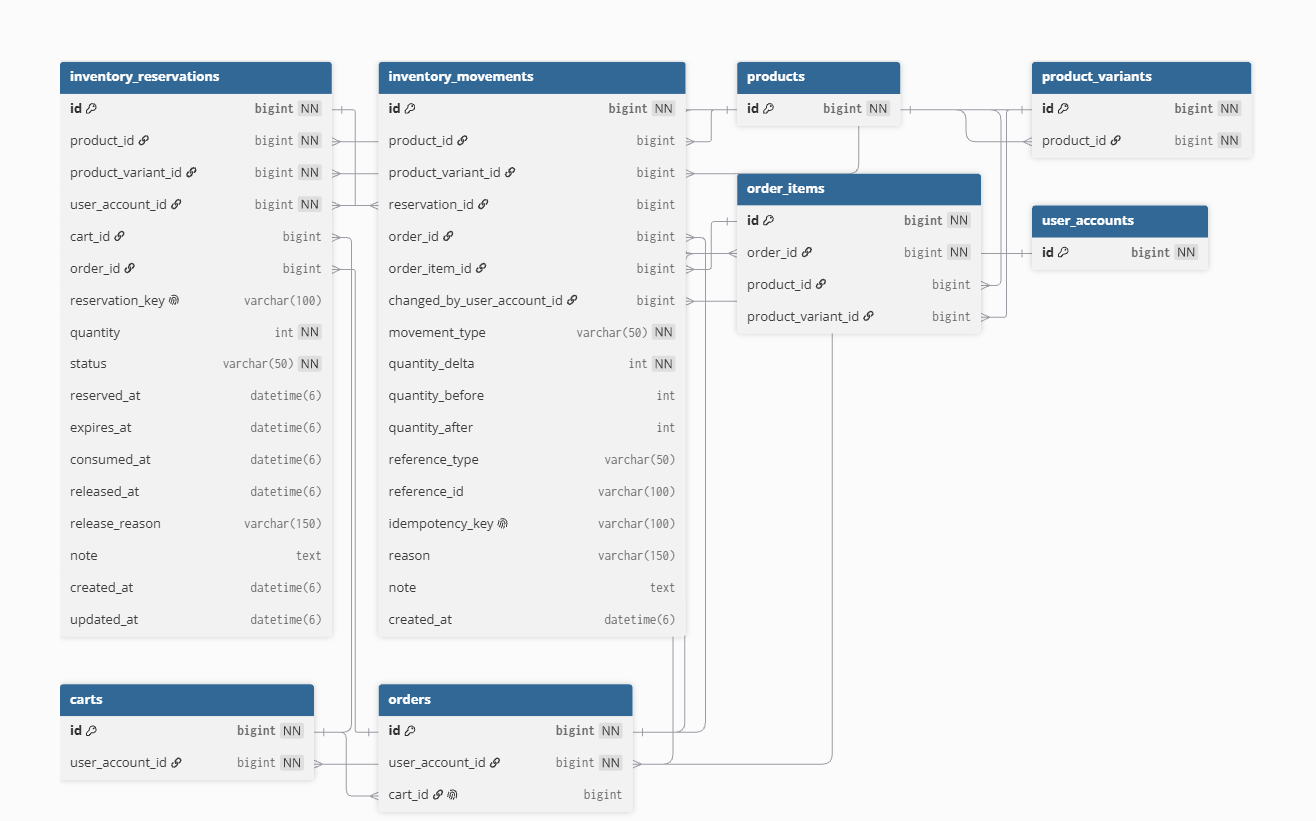
\includegraphics[
        width=\textwidth,
        height=0.72\textheight,
        keepaspectratio
    ]{Images/Thietkehethong/Quản lý kho.png}
    \caption{Sơ đồ dữ liệu quản lý kho}
    \label{fig:database-inventory}
\end{figure}

Theo Hình~\ref{fig:database-inventory},
\texttt{inventory\_reservations} biểu diễn phần tồn kho được giữ cho một người
dùng trong ngữ cảnh giỏ hàng hoặc đơn hàng. Mọi thay đổi tương ứng được ghi vào
\texttt{inventory\_movements} cùng lượng trước--sau, loại biến động và khóa
idempotency. Các bảng sản phẩm, giỏ hàng, đơn hàng và người dùng xuất hiện ở dạng
tham chiếu nhằm thể hiện nguồn phát sinh nghiệp vụ mà không lặp lại toàn bộ miền
dữ liệu liên quan.

Bảng~\ref{tab:data-summary-inventory} tóm tắt chức năng của các bảng trong nhóm. Chỉ các bảng cốt lõi, đại diện trực tiếp cho luồng nghiệp vụ chính, được mô tả chi tiết trường dữ liệu.

\begin{longtable}{|>{\RaggedRight\arraybackslash}p{0.34\textwidth}|>{\RaggedRight\arraybackslash}p{0.56\textwidth}|}
    \caption{Các bảng thuộc nhóm quản lý kho}
    \label{tab:data-summary-inventory} \\
    \hline
    \textbf{Tên bảng} & \textbf{Chức năng} \\
    \hline
    \endfirsthead
    \multicolumn{2}{c}{\tablename\ \thetable\ (tiếp theo)} \\
    \hline
    \textbf{Tên bảng} & \textbf{Chức năng} \\
    \hline
    \endhead
    \texttt{inventory\_reservations} & Giữ tồn kho. \\
    \hline
    \texttt{inventory\_movements} & Biến động tồn kho. \\
    \hline
\end{longtable}

\paragraph{Các bảng cốt lõi.}

\begin{longtable}{|>{\RaggedRight\arraybackslash}p{0.25\textwidth}|>{\RaggedRight\arraybackslash}p{0.20\textwidth}|>{\RaggedRight\arraybackslash}p{0.45\textwidth}|}
    \caption{Mô tả chi tiết bảng \texttt{inventory\_reservations} (Giữ tồn kho)}
    \label{tab:data-dictionary-inventory-reservations} \\
    \hline
    \textbf{Tên trường} & \textbf{Kiểu dữ liệu} & \textbf{Mô tả} \\
    \hline
    \endfirsthead
    \multicolumn{3}{c}{\tablename\ \thetable\ (tiếp theo)} \\
    \hline
    \textbf{Tên trường} & \textbf{Kiểu dữ liệu} & \textbf{Mô tả} \\
    \hline
    \endhead
    \texttt{\seqsplit{id}} & \texttt{bigint} & Khóa chính tự tăng. \\
        \hline
        \texttt{\seqsplit{product\_id}} & \texttt{bigint} & Khóa ngoại tham chiếu \texttt{products.id}; bắt buộc. \\
        \hline
        \texttt{\seqsplit{product\_variant\_id}} & \texttt{bigint} & Khóa ngoại tham chiếu \texttt{product\_variants.id}; bắt buộc. \\
        \hline
        \texttt{\seqsplit{user\_account\_id}} & \texttt{bigint} & Khóa ngoại tham chiếu \texttt{user\_accounts.id}; bắt buộc. \\
        \hline
        \texttt{\seqsplit{cart\_id}} & \texttt{bigint} & Khóa ngoại tham chiếu \texttt{carts.id}. \\
        \hline
        \texttt{\seqsplit{order\_id}} & \texttt{bigint} & Khóa ngoại tham chiếu \texttt{orders.id}. \\
        \hline
        \texttt{\seqsplit{reservation\_key}} & \texttt{varchar(100)} & Khóa duy nhất chống giữ tồn kho trùng; duy nhất. \\
        \hline
        \texttt{\seqsplit{quantity}} & \texttt{int} & Số lượng; bắt buộc. \\
        \hline
        \texttt{\seqsplit{status}} & \texttt{varchar(50)} & Trạng thái hiện tại; bắt buộc. \\
        \hline
        \texttt{\seqsplit{reserved\_at}} & \texttt{datetime(6)} & Thời điểm giữ hàng. \\
        \hline
        \texttt{\seqsplit{expires\_at}} & \texttt{datetime(6)} & Thời điểm hết hiệu lực. \\
        \hline
        \texttt{\seqsplit{consumed\_at}} & \texttt{datetime(6)} & Thời điểm phần giữ hàng được sử dụng. \\
        \hline
        \texttt{\seqsplit{released\_at}} & \texttt{datetime(6)} & Thời điểm giải phóng phần giữ hàng. \\
        \hline
        \texttt{\seqsplit{release\_reason}} & \texttt{varchar(150)} & Lý do giải phóng. \\
        \hline
        \texttt{\seqsplit{note}} & \texttt{text} & Ghi chú. \\
        \hline
        \texttt{\seqsplit{created\_at}} & \texttt{datetime(6)} & Thời điểm tạo bản ghi. \\
        \hline
        \texttt{\seqsplit{updated\_at}} & \texttt{datetime(6)} & Thời điểm cập nhật gần nhất. \\
        \hline
\end{longtable}

\begin{longtable}{|>{\RaggedRight\arraybackslash}p{0.25\textwidth}|>{\RaggedRight\arraybackslash}p{0.20\textwidth}|>{\RaggedRight\arraybackslash}p{0.45\textwidth}|}
    \caption{Mô tả chi tiết bảng \texttt{inventory\_movements} (Biến động tồn kho)}
    \label{tab:data-dictionary-inventory-movements} \\
    \hline
    \textbf{Tên trường} & \textbf{Kiểu dữ liệu} & \textbf{Mô tả} \\
    \hline
    \endfirsthead
    \multicolumn{3}{c}{\tablename\ \thetable\ (tiếp theo)} \\
    \hline
    \textbf{Tên trường} & \textbf{Kiểu dữ liệu} & \textbf{Mô tả} \\
    \hline
    \endhead
    \texttt{\seqsplit{id}} & \texttt{bigint} & Khóa chính tự tăng. \\
        \hline
        \texttt{\seqsplit{product\_id}} & \texttt{bigint} & Khóa ngoại tham chiếu \texttt{products.id}. \\
        \hline
        \texttt{\seqsplit{product\_variant\_id}} & \texttt{bigint} & Khóa ngoại tham chiếu \texttt{product\_variants.id}. \\
        \hline
        \texttt{\seqsplit{reservation\_id}} & \texttt{bigint} & Khóa ngoại tham chiếu \texttt{inventory\_reservations.id}. \\
        \hline
        \texttt{\seqsplit{order\_id}} & \texttt{bigint} & Khóa ngoại tham chiếu \texttt{orders.id}. \\
        \hline
        \texttt{\seqsplit{order\_item\_id}} & \texttt{bigint} & Khóa ngoại tham chiếu \texttt{order\_items.id}. \\
        \hline
        \texttt{\seqsplit{changed\_by\_user\_account\_id}} & \texttt{bigint} & Khóa ngoại tham chiếu \texttt{user\_accounts.id}. \\
        \hline
        \texttt{\seqsplit{movement\_type}} & \texttt{varchar(50)} & Loại biến động tồn kho; bắt buộc. \\
        \hline
        \texttt{\seqsplit{quantity\_delta}} & \texttt{int} & Lượng tồn kho thay đổi; bắt buộc. \\
        \hline
        \texttt{\seqsplit{quantity\_before}} & \texttt{int} & Số lượng trước biến động. \\
        \hline
        \texttt{\seqsplit{quantity\_after}} & \texttt{int} & Số lượng sau biến động. \\
        \hline
        \texttt{\seqsplit{reference\_type}} & \texttt{varchar(50)} & Loại đối tượng nghiệp vụ tham chiếu. \\
        \hline
        \texttt{\seqsplit{reference\_id}} & \texttt{varchar(100)} & Định danh đối tượng nghiệp vụ tham chiếu. \\
        \hline
        \texttt{\seqsplit{idempotency\_key}} & \texttt{varchar(100)} & Khóa duy nhất chống xử lý lặp; duy nhất. \\
        \hline
        \texttt{\seqsplit{reason}} & \texttt{varchar(150)} & Lý do. \\
        \hline
        \texttt{\seqsplit{note}} & \texttt{text} & Ghi chú. \\
        \hline
        \texttt{\seqsplit{created\_at}} & \texttt{datetime(6)} & Thời điểm tạo bản ghi. \\
        \hline
\end{longtable}



\subsubsection{Nhóm dữ liệu giỏ hàng và tương tác khách hàng}

Nhóm này lưu trạng thái giỏ hàng, các mặt hàng khách đã chọn, danh sách yêu thích,
đánh giá sản phẩm và nội dung blog phục vụ tương tác. Thông tin tổng hợp đánh giá
được tách khỏi đánh giá chi tiết để việc hiển thị số lượng và điểm trung bình
không phải tính lại trên toàn bộ dữ liệu sau mỗi truy vấn.

\begin{figure}[H]
    \centering
    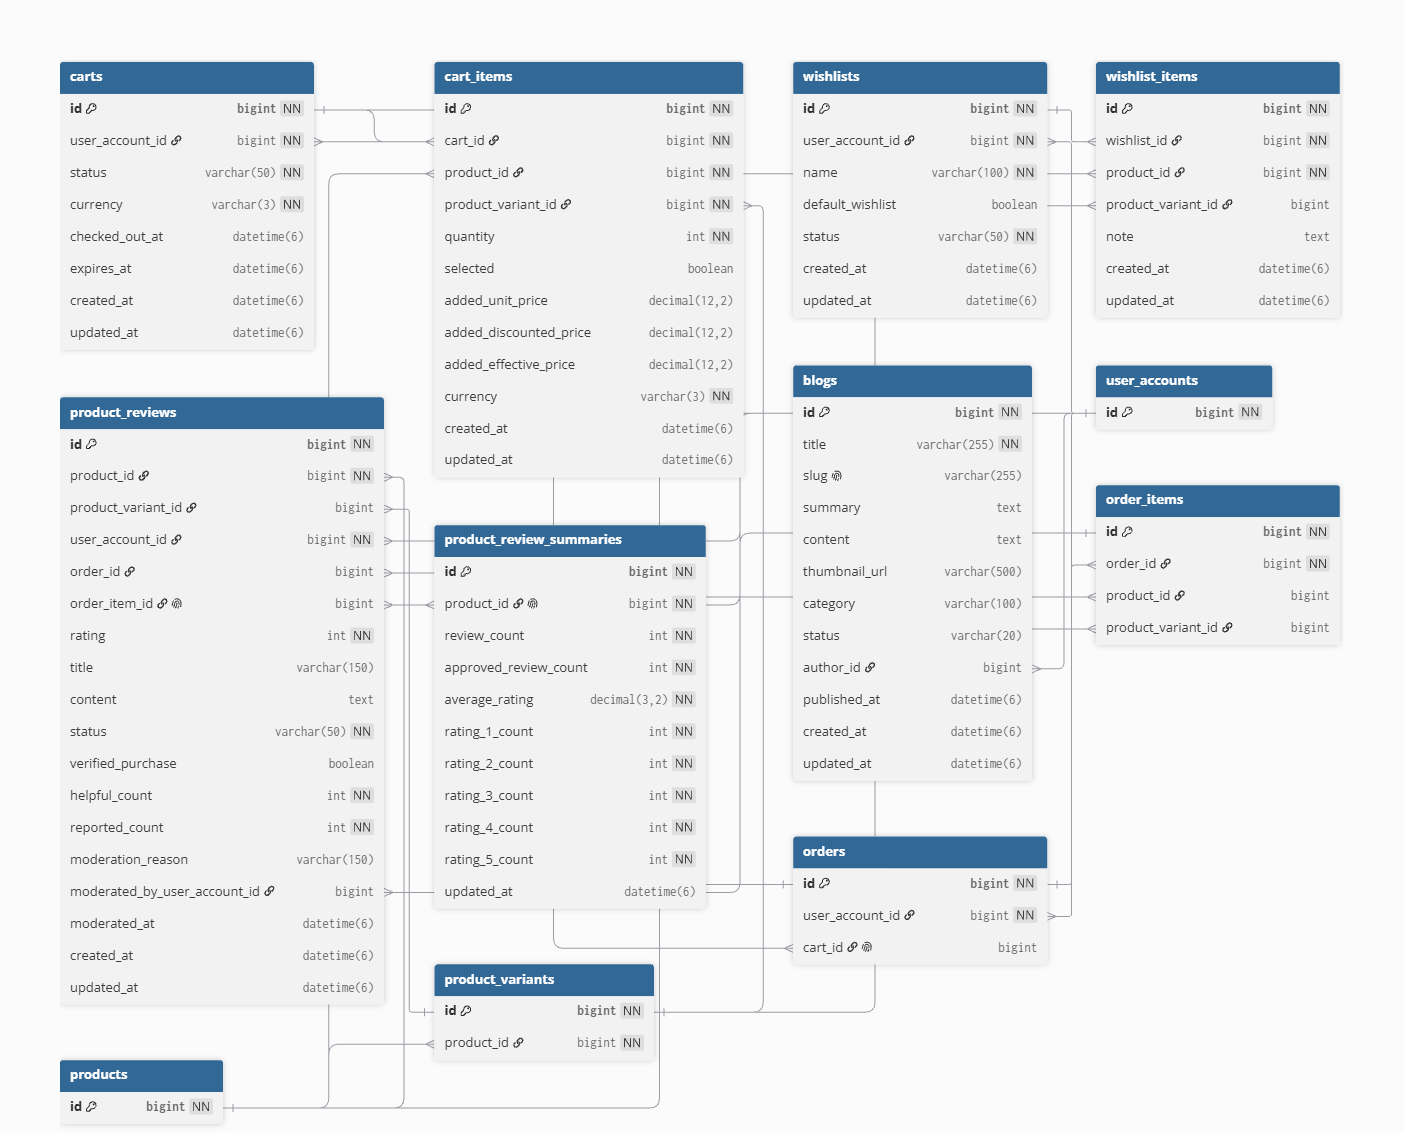
\includegraphics[
        width=\textwidth,
        height=0.72\textheight,
        keepaspectratio
    ]{Images/Thietkehethong/Giỏ hàng và tương tác khách hàng.png}
    \caption{Sơ đồ dữ liệu giỏ hàng và tương tác khách hàng}
    \label{fig:database-cart-engagement}
\end{figure}

Hình~\ref{fig:database-cart-engagement} tập hợp các dữ liệu phát sinh từ quá
trình tương tác của khách hàng. Giỏ hàng và danh sách yêu thích đều được tổ chức
theo mô hình bảng đầu mục--chi tiết. Đánh giá liên kết với người dùng, sản phẩm
và dòng đơn hàng để xác minh giao dịch mua, trong khi
\texttt{product\_review\_summaries} lưu kết quả tổng hợp phục vụ truy vấn đọc.
Bài viết blog liên kết tùy chọn với tài khoản tác giả và không phụ thuộc vào vòng
đời mua hàng.

Bảng~\ref{tab:data-summary-cart-engagement} tóm tắt chức năng của các bảng trong nhóm. Chỉ các bảng cốt lõi, đại diện trực tiếp cho luồng nghiệp vụ chính, được mô tả chi tiết trường dữ liệu.

\begin{longtable}{|>{\RaggedRight\arraybackslash}p{0.34\textwidth}|>{\RaggedRight\arraybackslash}p{0.56\textwidth}|}
    \caption{Các bảng thuộc nhóm giỏ hàng và tương tác khách hàng}
    \label{tab:data-summary-cart-engagement} \\
    \hline
    \textbf{Tên bảng} & \textbf{Chức năng} \\
    \hline
    \endfirsthead
    \multicolumn{2}{c}{\tablename\ \thetable\ (tiếp theo)} \\
    \hline
    \textbf{Tên bảng} & \textbf{Chức năng} \\
    \hline
    \endhead
    \texttt{carts} & Giỏ hàng. \\
    \hline
    \texttt{cart\_items} & Chi tiết giỏ hàng. \\
    \hline
    \texttt{wishlists} & Danh sách yêu thích. \\
    \hline
    \texttt{wishlist\_items} & Chi tiết danh sách yêu thích. \\
    \hline
    \texttt{product\_reviews} & Đánh giá sản phẩm. \\
    \hline
    \texttt{product\_review\_summaries} & Tổng hợp đánh giá sản phẩm. \\
    \hline
    \texttt{blogs} & Bài viết. \\
    \hline
\end{longtable}

\paragraph{Các bảng cốt lõi.}

\begin{longtable}{|>{\RaggedRight\arraybackslash}p{0.25\textwidth}|>{\RaggedRight\arraybackslash}p{0.20\textwidth}|>{\RaggedRight\arraybackslash}p{0.45\textwidth}|}
    \caption{Mô tả chi tiết bảng \texttt{carts} (Giỏ hàng)}
    \label{tab:data-dictionary-carts} \\
    \hline
    \textbf{Tên trường} & \textbf{Kiểu dữ liệu} & \textbf{Mô tả} \\
    \hline
    \endfirsthead
    \multicolumn{3}{c}{\tablename\ \thetable\ (tiếp theo)} \\
    \hline
    \textbf{Tên trường} & \textbf{Kiểu dữ liệu} & \textbf{Mô tả} \\
    \hline
    \endhead
    \texttt{\seqsplit{id}} & \texttt{bigint} & Khóa chính tự tăng. \\
        \hline
        \texttt{\seqsplit{user\_account\_id}} & \texttt{bigint} & Khóa ngoại tham chiếu \texttt{user\_accounts.id}; bắt buộc. \\
        \hline
        \texttt{\seqsplit{status}} & \texttt{varchar(50)} & Trạng thái hiện tại; bắt buộc. \\
        \hline
        \texttt{\seqsplit{currency}} & \texttt{varchar(3)} & Mã tiền tệ ISO 4217; bắt buộc. \\
        \hline
        \texttt{\seqsplit{checked\_out\_at}} & \texttt{datetime(6)} & Thời điểm giỏ hàng được chuyển thành đơn. \\
        \hline
        \texttt{\seqsplit{expires\_at}} & \texttt{datetime(6)} & Thời điểm hết hiệu lực. \\
        \hline
        \texttt{\seqsplit{created\_at}} & \texttt{datetime(6)} & Thời điểm tạo bản ghi. \\
        \hline
        \texttt{\seqsplit{updated\_at}} & \texttt{datetime(6)} & Thời điểm cập nhật gần nhất. \\
        \hline
\end{longtable}

\begin{longtable}{|>{\RaggedRight\arraybackslash}p{0.25\textwidth}|>{\RaggedRight\arraybackslash}p{0.20\textwidth}|>{\RaggedRight\arraybackslash}p{0.45\textwidth}|}
    \caption{Mô tả chi tiết bảng \texttt{cart\_items} (Chi tiết giỏ hàng)}
    \label{tab:data-dictionary-cart-items} \\
    \hline
    \textbf{Tên trường} & \textbf{Kiểu dữ liệu} & \textbf{Mô tả} \\
    \hline
    \endfirsthead
    \multicolumn{3}{c}{\tablename\ \thetable\ (tiếp theo)} \\
    \hline
    \textbf{Tên trường} & \textbf{Kiểu dữ liệu} & \textbf{Mô tả} \\
    \hline
    \endhead
    \texttt{\seqsplit{id}} & \texttt{bigint} & Khóa chính tự tăng. \\
        \hline
        \texttt{\seqsplit{cart\_id}} & \texttt{bigint} & Khóa ngoại tham chiếu \texttt{carts.id}; bắt buộc. \\
        \hline
        \texttt{\seqsplit{product\_id}} & \texttt{bigint} & Khóa ngoại tham chiếu \texttt{products.id}; bắt buộc. \\
        \hline
        \texttt{\seqsplit{product\_variant\_id}} & \texttt{bigint} & Khóa ngoại tham chiếu \texttt{product\_variants.id}; bắt buộc. \\
        \hline
        \texttt{\seqsplit{quantity}} & \texttt{int} & Số lượng; bắt buộc. \\
        \hline
        \texttt{\seqsplit{selected}} & \texttt{boolean} & Cho biết mặt hàng được chọn. \\
        \hline
        \texttt{\seqsplit{added\_unit\_price}} & \texttt{decimal(12,2)} & Đơn giá tại thời điểm thêm vào giỏ. \\
        \hline
        \texttt{\seqsplit{added\_discounted\_price}} & \texttt{decimal(12,2)} & Đơn giá sau giảm tại thời điểm thêm vào giỏ. \\
        \hline
        \texttt{\seqsplit{added\_effective\_price}} & \texttt{decimal(12,2)} & Đơn giá hiệu lực tại thời điểm thêm vào giỏ. \\
        \hline
        \texttt{\seqsplit{currency}} & \texttt{varchar(3)} & Mã tiền tệ ISO 4217; bắt buộc. \\
        \hline
        \texttt{\seqsplit{created\_at}} & \texttt{datetime(6)} & Thời điểm tạo bản ghi. \\
        \hline
        \texttt{\seqsplit{updated\_at}} & \texttt{datetime(6)} & Thời điểm cập nhật gần nhất. \\
        \hline
\end{longtable}

\begin{longtable}{|>{\RaggedRight\arraybackslash}p{0.25\textwidth}|>{\RaggedRight\arraybackslash}p{0.20\textwidth}|>{\RaggedRight\arraybackslash}p{0.45\textwidth}|}
    \caption{Mô tả chi tiết bảng \texttt{product\_reviews} (Đánh giá sản phẩm)}
    \label{tab:data-dictionary-product-reviews} \\
    \hline
    \textbf{Tên trường} & \textbf{Kiểu dữ liệu} & \textbf{Mô tả} \\
    \hline
    \endfirsthead
    \multicolumn{3}{c}{\tablename\ \thetable\ (tiếp theo)} \\
    \hline
    \textbf{Tên trường} & \textbf{Kiểu dữ liệu} & \textbf{Mô tả} \\
    \hline
    \endhead
    \texttt{\seqsplit{id}} & \texttt{bigint} & Khóa chính tự tăng. \\
        \hline
        \texttt{\seqsplit{product\_id}} & \texttt{bigint} & Khóa ngoại tham chiếu \texttt{products.id}; bắt buộc. \\
        \hline
        \texttt{\seqsplit{product\_variant\_id}} & \texttt{bigint} & Khóa ngoại tham chiếu \texttt{product\_variants.id}. \\
        \hline
        \texttt{\seqsplit{user\_account\_id}} & \texttt{bigint} & Khóa ngoại tham chiếu \texttt{user\_accounts.id}; bắt buộc. \\
        \hline
        \texttt{\seqsplit{order\_id}} & \texttt{bigint} & Khóa ngoại tham chiếu \texttt{orders.id}. \\
        \hline
        \texttt{\seqsplit{order\_item\_id}} & \texttt{bigint} & Khóa ngoại tham chiếu \texttt{order\_items.id}; duy nhất. \\
        \hline
        \texttt{\seqsplit{rating}} & \texttt{int} & Điểm đánh giá; bắt buộc. \\
        \hline
        \texttt{\seqsplit{title}} & \texttt{varchar(150)} & Tiêu đề. \\
        \hline
        \texttt{\seqsplit{content}} & \texttt{text} & Nội dung. \\
        \hline
        \texttt{\seqsplit{status}} & \texttt{varchar(50)} & Trạng thái hiện tại; bắt buộc. \\
        \hline
        \texttt{\seqsplit{verified\_purchase}} & \texttt{boolean} & Cho biết đánh giá phát sinh từ giao dịch đã xác minh. \\
        \hline
        \texttt{\seqsplit{helpful\_count}} & \texttt{int} & Số lượt đánh dấu hữu ích; bắt buộc. \\
        \hline
        \texttt{\seqsplit{reported\_count}} & \texttt{int} & Số lượt báo cáo; bắt buộc. \\
        \hline
        \texttt{\seqsplit{moderation\_reason}} & \texttt{varchar(150)} & Lý do kiểm duyệt. \\
        \hline
        \texttt{\seqsplit{moderated\_by\_user\_account\_id}} & \texttt{bigint} & Khóa ngoại tham chiếu \texttt{user\_accounts.id}. \\
        \hline
        \texttt{\seqsplit{moderated\_at}} & \texttt{datetime(6)} & Thời điểm kiểm duyệt. \\
        \hline
        \texttt{\seqsplit{created\_at}} & \texttt{datetime(6)} & Thời điểm tạo bản ghi. \\
        \hline
        \texttt{\seqsplit{updated\_at}} & \texttt{datetime(6)} & Thời điểm cập nhật gần nhất. \\
        \hline
\end{longtable}



\subsubsection{Nhóm dữ liệu đơn hàng và vận chuyển}

Nhóm đơn hàng lưu kết quả của quá trình mua sắm, các dòng hàng, bản chụp địa chỉ
nhận hàng và lịch sử chuyển trạng thái. Giá, tên và thuộc tính cần thiết của sản
phẩm được chụp lại trong \texttt{order\_items}; do đó nội dung đơn đã phát sinh
không bị thay đổi khi dữ liệu sản phẩm hiện hành được cập nhật hoặc xóa.

\begin{figure}[H]
    \centering
    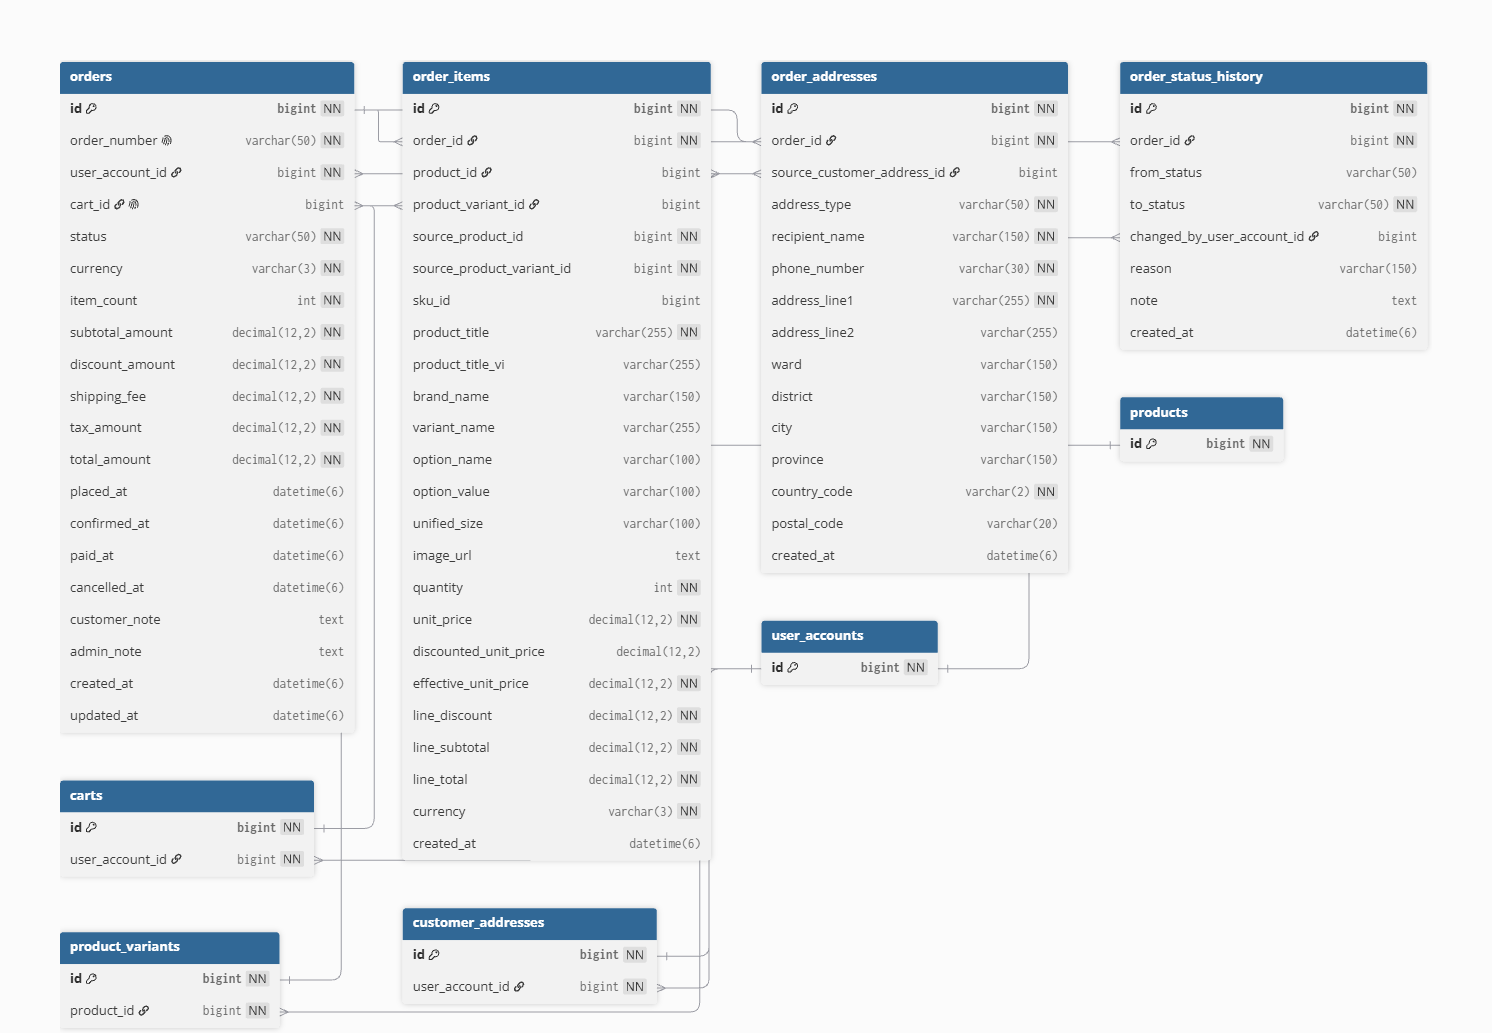
\includegraphics[
        width=\textwidth,
        height=0.72\textheight,
        keepaspectratio
    ]{Images/Thietkehethong/Đơn hàng và vận chuyển.png}
    \caption{Sơ đồ dữ liệu đơn hàng và vận chuyển}
    \label{fig:database-order-shipping}
\end{figure}

Trong Hình~\ref{fig:database-order-shipping}, \texttt{orders} liên kết một--nhiều
với các dòng hàng, địa chỉ chụp tại thời điểm đặt và lịch sử trạng thái. Liên kết
đến sản phẩm và biến thể được phép rỗng để đơn hàng cũ vẫn tồn tại khi dữ liệu
danh mục thay đổi. Tương tự, \texttt{order\_addresses} giữ bản sao địa chỉ giao
nhận thay vì phụ thuộc hoàn toàn vào địa chỉ hiện hành trong hồ sơ khách hàng.

Bảng~\ref{tab:data-summary-order-shipping} tóm tắt chức năng của các bảng trong nhóm. Chỉ các bảng cốt lõi, đại diện trực tiếp cho luồng nghiệp vụ chính, được mô tả chi tiết trường dữ liệu.

\begin{longtable}{|>{\RaggedRight\arraybackslash}p{0.34\textwidth}|>{\RaggedRight\arraybackslash}p{0.56\textwidth}|}
    \caption{Các bảng thuộc nhóm đơn hàng và vận chuyển}
    \label{tab:data-summary-order-shipping} \\
    \hline
    \textbf{Tên bảng} & \textbf{Chức năng} \\
    \hline
    \endfirsthead
    \multicolumn{2}{c}{\tablename\ \thetable\ (tiếp theo)} \\
    \hline
    \textbf{Tên bảng} & \textbf{Chức năng} \\
    \hline
    \endhead
    \texttt{orders} & Đơn hàng. \\
    \hline
    \texttt{order\_items} & Chi tiết đơn hàng. \\
    \hline
    \texttt{order\_addresses} & Địa chỉ đơn hàng. \\
    \hline
    \texttt{order\_status\_history} & Lịch sử trạng thái đơn hàng. \\
    \hline
\end{longtable}

\paragraph{Các bảng cốt lõi.}

\begin{longtable}{|>{\RaggedRight\arraybackslash}p{0.25\textwidth}|>{\RaggedRight\arraybackslash}p{0.20\textwidth}|>{\RaggedRight\arraybackslash}p{0.45\textwidth}|}
    \caption{Mô tả chi tiết bảng \texttt{orders} (Đơn hàng)}
    \label{tab:data-dictionary-orders} \\
    \hline
    \textbf{Tên trường} & \textbf{Kiểu dữ liệu} & \textbf{Mô tả} \\
    \hline
    \endfirsthead
    \multicolumn{3}{c}{\tablename\ \thetable\ (tiếp theo)} \\
    \hline
    \textbf{Tên trường} & \textbf{Kiểu dữ liệu} & \textbf{Mô tả} \\
    \hline
    \endhead
    \texttt{\seqsplit{id}} & \texttt{bigint} & Khóa chính tự tăng. \\
        \hline
        \texttt{\seqsplit{order\_number}} & \texttt{varchar(50)} & Mã đơn hàng duy nhất; bắt buộc; duy nhất. \\
        \hline
        \texttt{\seqsplit{user\_account\_id}} & \texttt{bigint} & Khóa ngoại tham chiếu \texttt{user\_accounts.id}; bắt buộc. \\
        \hline
        \texttt{\seqsplit{cart\_id}} & \texttt{bigint} & Khóa ngoại tham chiếu \texttt{carts.id}; duy nhất. \\
        \hline
        \texttt{\seqsplit{status}} & \texttt{varchar(50)} & Trạng thái hiện tại; bắt buộc. \\
        \hline
        \texttt{\seqsplit{currency}} & \texttt{varchar(3)} & Mã tiền tệ ISO 4217; bắt buộc. \\
        \hline
        \texttt{\seqsplit{item\_count}} & \texttt{int} & Tổng số mặt hàng trong đơn; bắt buộc. \\
        \hline
        \texttt{\seqsplit{subtotal\_amount}} & \texttt{decimal(12,2)} & Tạm tính trước giảm giá và phí; bắt buộc. \\
        \hline
        \texttt{\seqsplit{discount\_amount}} & \texttt{decimal(12,2)} & Tổng số tiền được giảm; bắt buộc. \\
        \hline
        \texttt{\seqsplit{shipping\_fee}} & \texttt{decimal(12,2)} & Phí vận chuyển; bắt buộc. \\
        \hline
        \texttt{\seqsplit{tax\_amount}} & \texttt{decimal(12,2)} & Tiền thuế; bắt buộc. \\
        \hline
        \texttt{\seqsplit{total\_amount}} & \texttt{decimal(12,2)} & Tổng tiền phải thanh toán; bắt buộc. \\
        \hline
        \texttt{\seqsplit{placed\_at}} & \texttt{datetime(6)} & Thời điểm đặt hàng. \\
        \hline
        \texttt{\seqsplit{confirmed\_at}} & \texttt{datetime(6)} & Thời điểm xác nhận đơn. \\
        \hline
        \texttt{\seqsplit{paid\_at}} & \texttt{datetime(6)} & Thời điểm thanh toán thành công. \\
        \hline
        \texttt{\seqsplit{cancelled\_at}} & \texttt{datetime(6)} & Thời điểm hủy. \\
        \hline
        \texttt{\seqsplit{customer\_note}} & \texttt{text} & Ghi chú của khách hàng. \\
        \hline
        \texttt{\seqsplit{admin\_note}} & \texttt{text} & Ghi chú quản trị. \\
        \hline
        \texttt{\seqsplit{created\_at}} & \texttt{datetime(6)} & Thời điểm tạo bản ghi. \\
        \hline
        \texttt{\seqsplit{updated\_at}} & \texttt{datetime(6)} & Thời điểm cập nhật gần nhất. \\
        \hline
\end{longtable}

\begin{longtable}{|>{\RaggedRight\arraybackslash}p{0.25\textwidth}|>{\RaggedRight\arraybackslash}p{0.20\textwidth}|>{\RaggedRight\arraybackslash}p{0.45\textwidth}|}
    \caption{Mô tả chi tiết bảng \texttt{order\_items} (Chi tiết đơn hàng)}
    \label{tab:data-dictionary-order-items} \\
    \hline
    \textbf{Tên trường} & \textbf{Kiểu dữ liệu} & \textbf{Mô tả} \\
    \hline
    \endfirsthead
    \multicolumn{3}{c}{\tablename\ \thetable\ (tiếp theo)} \\
    \hline
    \textbf{Tên trường} & \textbf{Kiểu dữ liệu} & \textbf{Mô tả} \\
    \hline
    \endhead
    \texttt{\seqsplit{id}} & \texttt{bigint} & Khóa chính tự tăng. \\
        \hline
        \texttt{\seqsplit{order\_id}} & \texttt{bigint} & Khóa ngoại tham chiếu \texttt{orders.id}; bắt buộc. \\
        \hline
        \texttt{\seqsplit{product\_id}} & \texttt{bigint} & Khóa ngoại tham chiếu \texttt{products.id}. \\
        \hline
        \texttt{\seqsplit{product\_variant\_id}} & \texttt{bigint} & Khóa ngoại tham chiếu \texttt{product\_variants.id}. \\
        \hline
        \texttt{\seqsplit{source\_product\_id}} & \texttt{bigint} & Định danh sản phẩm nguồn được chụp tại thời điểm mua; bắt buộc. \\
        \hline
        \texttt{\seqsplit{source\_product\_variant\_id}} & \texttt{bigint} & Định danh biến thể nguồn được chụp tại thời điểm mua; bắt buộc. \\
        \hline
        \texttt{\seqsplit{sku\_id}} & \texttt{bigint} & Định danh SKU. \\
        \hline
        \texttt{\seqsplit{product\_title}} & \texttt{varchar(255)} & Tên sản phẩm được chụp tại thời điểm mua; bắt buộc. \\
        \hline
        \texttt{\seqsplit{product\_title\_vi}} & \texttt{varchar(255)} & Tên sản phẩm tiếng Việt được chụp tại thời điểm mua. \\
        \hline
        \texttt{\seqsplit{brand\_name}} & \texttt{varchar(150)} & Tên thương hiệu. \\
        \hline
        \texttt{\seqsplit{variant\_name}} & \texttt{varchar(255)} & Tên biến thể. \\
        \hline
        \texttt{\seqsplit{option\_name}} & \texttt{varchar(100)} & Tên tùy chọn biến thể. \\
        \hline
        \texttt{\seqsplit{option\_value}} & \texttt{varchar(100)} & Giá trị tùy chọn biến thể. \\
        \hline
        \texttt{\seqsplit{unified\_size}} & \texttt{varchar(100)} & Kích cỡ đã chuẩn hóa. \\
        \hline
        \texttt{\seqsplit{image\_url}} & \texttt{text} & Đường dẫn hình ảnh. \\
        \hline
        \texttt{\seqsplit{quantity}} & \texttt{int} & Số lượng; bắt buộc. \\
        \hline
        \texttt{\seqsplit{unit\_price}} & \texttt{decimal(12,2)} & Đơn giá gốc; bắt buộc. \\
        \hline
        \texttt{\seqsplit{discounted\_unit\_price}} & \texttt{decimal(12,2)} & Đơn giá sau giảm. \\
        \hline
        \texttt{\seqsplit{effective\_unit\_price}} & \texttt{decimal(12,2)} & Đơn giá thực tế áp dụng; bắt buộc. \\
        \hline
        \texttt{\seqsplit{line\_discount}} & \texttt{decimal(12,2)} & Tiền giảm của dòng hàng; bắt buộc. \\
        \hline
        \texttt{\seqsplit{line\_subtotal}} & \texttt{decimal(12,2)} & Tạm tính của dòng hàng; bắt buộc. \\
        \hline
        \texttt{\seqsplit{line\_total}} & \texttt{decimal(12,2)} & Thành tiền của dòng hàng; bắt buộc. \\
        \hline
        \texttt{\seqsplit{currency}} & \texttt{varchar(3)} & Mã tiền tệ ISO 4217; bắt buộc. \\
        \hline
        \texttt{\seqsplit{created\_at}} & \texttt{datetime(6)} & Thời điểm tạo bản ghi. \\
        \hline
\end{longtable}

\begin{longtable}{|>{\RaggedRight\arraybackslash}p{0.25\textwidth}|>{\RaggedRight\arraybackslash}p{0.20\textwidth}|>{\RaggedRight\arraybackslash}p{0.45\textwidth}|}
    \caption{Mô tả chi tiết bảng \texttt{order\_status\_history} (Lịch sử trạng thái đơn hàng)}
    \label{tab:data-dictionary-order-status-history} \\
    \hline
    \textbf{Tên trường} & \textbf{Kiểu dữ liệu} & \textbf{Mô tả} \\
    \hline
    \endfirsthead
    \multicolumn{3}{c}{\tablename\ \thetable\ (tiếp theo)} \\
    \hline
    \textbf{Tên trường} & \textbf{Kiểu dữ liệu} & \textbf{Mô tả} \\
    \hline
    \endhead
    \texttt{\seqsplit{id}} & \texttt{bigint} & Khóa chính tự tăng. \\
        \hline
        \texttt{\seqsplit{order\_id}} & \texttt{bigint} & Khóa ngoại tham chiếu \texttt{orders.id}; bắt buộc. \\
        \hline
        \texttt{\seqsplit{from\_status}} & \texttt{varchar(50)} & Trạng thái trước khi chuyển. \\
        \hline
        \texttt{\seqsplit{to\_status}} & \texttt{varchar(50)} & Trạng thái sau khi chuyển; bắt buộc. \\
        \hline
        \texttt{\seqsplit{changed\_by\_user\_account\_id}} & \texttt{bigint} & Khóa ngoại tham chiếu \texttt{user\_accounts.id}. \\
        \hline
        \texttt{\seqsplit{reason}} & \texttt{varchar(150)} & Lý do. \\
        \hline
        \texttt{\seqsplit{note}} & \texttt{text} & Ghi chú. \\
        \hline
        \texttt{\seqsplit{created\_at}} & \texttt{datetime(6)} & Thời điểm tạo bản ghi. \\
        \hline
\end{longtable}



\subsubsection{Nhóm dữ liệu thanh toán và khuyến mãi}

Nhóm này quản lý khoản thanh toán của đơn hàng, từng giao dịch với nhà cung cấp,
sự kiện webhook và các chính sách giảm giá. Khuyến mãi có thể giới hạn theo sản
phẩm hoặc danh mục, trong khi lịch sử đổi coupon lưu bản chụp giá trị giảm và
trạng thái sử dụng để hỗ trợ kiểm tra, hủy hoặc hoàn tác đơn hàng.

\begin{figure}[H]
    \centering
    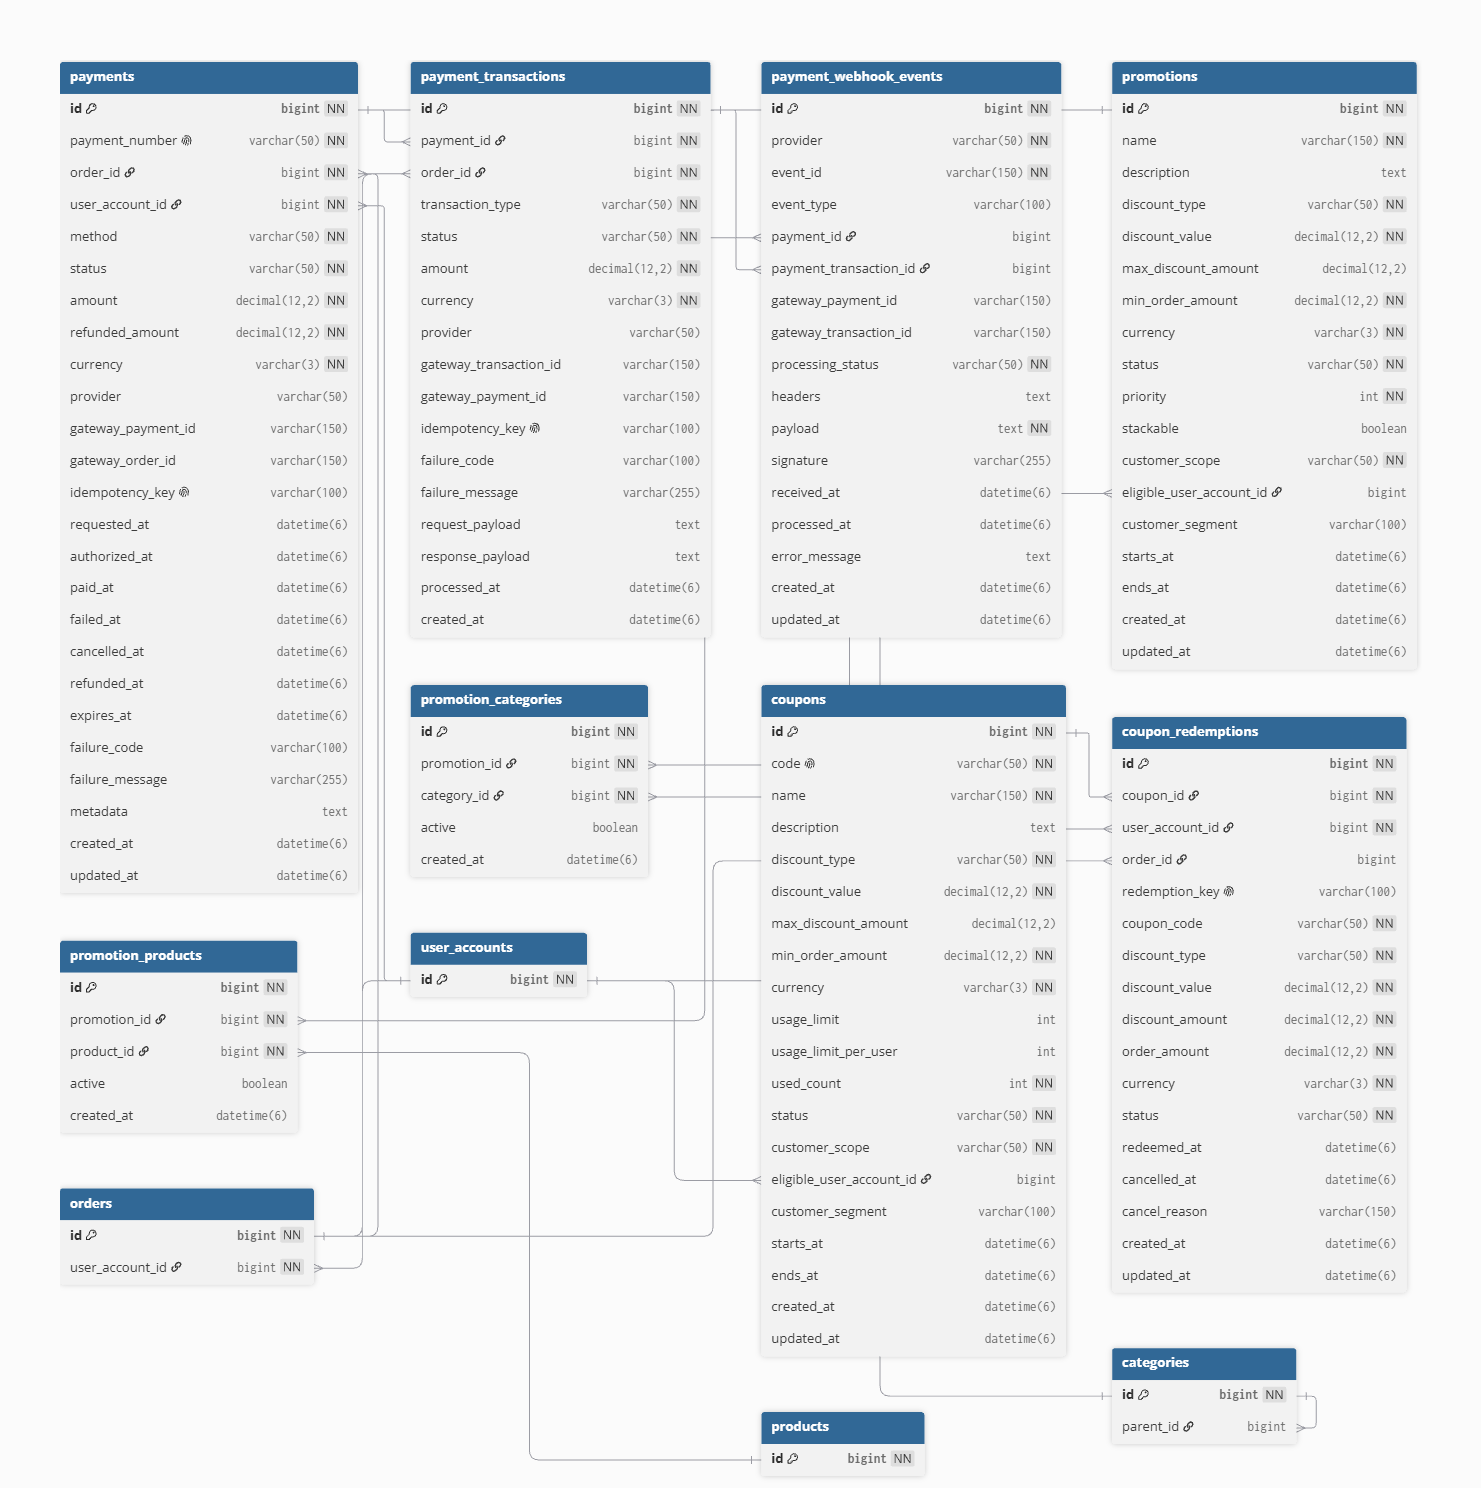
\includegraphics[
        width=\textwidth,
        height=0.72\textheight,
        keepaspectratio
    ]{Images/Thietkehethong/Thanh toán và khuyến mãi.png}
    \caption{Sơ đồ dữ liệu thanh toán và khuyến mãi}
    \label{fig:database-payment-promotion}
\end{figure}

Hình~\ref{fig:database-payment-promotion} thể hiện ba cụm quan hệ chính. Cụm
thanh toán liên kết \texttt{payments} với các lần giao dịch và sự kiện webhook
để hỗ trợ đối soát. Cụm khuyến mãi dùng các bảng liên kết để giới hạn phạm vi
theo sản phẩm hoặc danh mục. Cụm coupon ghi nhận lượt sử dụng theo người dùng và
đơn hàng, đồng thời chụp lại loại giảm, giá trị giảm và số tiền thực tế để bảo
toàn lịch sử tính giá.

Bảng~\ref{tab:data-summary-payment-promotion} tóm tắt chức năng của các bảng trong nhóm. Chỉ các bảng cốt lõi, đại diện trực tiếp cho luồng nghiệp vụ chính, được mô tả chi tiết trường dữ liệu.

\begin{longtable}{|>{\RaggedRight\arraybackslash}p{0.34\textwidth}|>{\RaggedRight\arraybackslash}p{0.56\textwidth}|}
    \caption{Các bảng thuộc nhóm thanh toán và khuyến mãi}
    \label{tab:data-summary-payment-promotion} \\
    \hline
    \textbf{Tên bảng} & \textbf{Chức năng} \\
    \hline
    \endfirsthead
    \multicolumn{2}{c}{\tablename\ \thetable\ (tiếp theo)} \\
    \hline
    \textbf{Tên bảng} & \textbf{Chức năng} \\
    \hline
    \endhead
    \texttt{payments} & Thanh toán. \\
    \hline
    \texttt{payment\_transactions} & Giao dịch thanh toán. \\
    \hline
    \texttt{payment\_webhook\_events} & Sự kiện webhook thanh toán. \\
    \hline
    \texttt{promotions} & Chương trình khuyến mãi. \\
    \hline
    \texttt{promotion\_products} & Sản phẩm áp dụng khuyến mãi. \\
    \hline
    \texttt{promotion\_categories} & Danh mục áp dụng khuyến mãi. \\
    \hline
    \texttt{coupons} & Mã giảm giá. \\
    \hline
    \texttt{coupon\_redemptions} & Lượt sử dụng mã giảm giá. \\
    \hline
\end{longtable}

\paragraph{Các bảng cốt lõi.}

\begin{longtable}{|>{\RaggedRight\arraybackslash}p{0.25\textwidth}|>{\RaggedRight\arraybackslash}p{0.20\textwidth}|>{\RaggedRight\arraybackslash}p{0.45\textwidth}|}
    \caption{Mô tả chi tiết bảng \texttt{payments} (Thanh toán)}
    \label{tab:data-dictionary-payments} \\
    \hline
    \textbf{Tên trường} & \textbf{Kiểu dữ liệu} & \textbf{Mô tả} \\
    \hline
    \endfirsthead
    \multicolumn{3}{c}{\tablename\ \thetable\ (tiếp theo)} \\
    \hline
    \textbf{Tên trường} & \textbf{Kiểu dữ liệu} & \textbf{Mô tả} \\
    \hline
    \endhead
    \texttt{\seqsplit{id}} & \texttt{bigint} & Khóa chính tự tăng. \\
        \hline
        \texttt{\seqsplit{payment\_number}} & \texttt{varchar(50)} & Mã thanh toán duy nhất; bắt buộc; duy nhất. \\
        \hline
        \texttt{\seqsplit{order\_id}} & \texttt{bigint} & Khóa ngoại tham chiếu \texttt{orders.id}; bắt buộc. \\
        \hline
        \texttt{\seqsplit{user\_account\_id}} & \texttt{bigint} & Khóa ngoại tham chiếu \texttt{user\_accounts.id}; bắt buộc. \\
        \hline
        \texttt{\seqsplit{method}} & \texttt{varchar(50)} & Phương thức thanh toán; bắt buộc. \\
        \hline
        \texttt{\seqsplit{status}} & \texttt{varchar(50)} & Trạng thái hiện tại; bắt buộc. \\
        \hline
        \texttt{\seqsplit{amount}} & \texttt{decimal(12,2)} & Số tiền; bắt buộc. \\
        \hline
        \texttt{\seqsplit{refunded\_amount}} & \texttt{decimal(12,2)} & Số tiền đã hoàn; bắt buộc. \\
        \hline
        \texttt{\seqsplit{currency}} & \texttt{varchar(3)} & Mã tiền tệ ISO 4217; bắt buộc. \\
        \hline
        \texttt{\seqsplit{provider}} & \texttt{varchar(50)} & Nhà cung cấp thanh toán. \\
        \hline
        \texttt{\seqsplit{gateway\_payment\_id}} & \texttt{varchar(150)} & Định danh thanh toán tại cổng. \\
        \hline
        \texttt{\seqsplit{gateway\_order\_id}} & \texttt{varchar(150)} & Định danh đơn hàng tại cổng. \\
        \hline
        \texttt{\seqsplit{idempotency\_key}} & \texttt{varchar(100)} & Khóa duy nhất chống xử lý lặp; duy nhất. \\
        \hline
        \texttt{\seqsplit{requested\_at}} & \texttt{datetime(6)} & Thời điểm yêu cầu thanh toán. \\
        \hline
        \texttt{\seqsplit{authorized\_at}} & \texttt{datetime(6)} & Thời điểm ủy quyền thanh toán. \\
        \hline
        \texttt{\seqsplit{paid\_at}} & \texttt{datetime(6)} & Thời điểm thanh toán thành công. \\
        \hline
        \texttt{\seqsplit{failed\_at}} & \texttt{datetime(6)} & Thời điểm thất bại. \\
        \hline
        \texttt{\seqsplit{cancelled\_at}} & \texttt{datetime(6)} & Thời điểm hủy. \\
        \hline
        \texttt{\seqsplit{refunded\_at}} & \texttt{datetime(6)} & Thời điểm hoàn tiền. \\
        \hline
        \texttt{\seqsplit{expires\_at}} & \texttt{datetime(6)} & Thời điểm hết hiệu lực. \\
        \hline
        \texttt{\seqsplit{failure\_code}} & \texttt{varchar(100)} & Mã lỗi. \\
        \hline
        \texttt{\seqsplit{failure\_message}} & \texttt{varchar(255)} & Thông báo lỗi. \\
        \hline
        \texttt{\seqsplit{metadata}} & \texttt{text} & Siêu dữ liệu bổ sung. \\
        \hline
        \texttt{\seqsplit{created\_at}} & \texttt{datetime(6)} & Thời điểm tạo bản ghi. \\
        \hline
        \texttt{\seqsplit{updated\_at}} & \texttt{datetime(6)} & Thời điểm cập nhật gần nhất. \\
        \hline
\end{longtable}

\begin{longtable}{|>{\RaggedRight\arraybackslash}p{0.25\textwidth}|>{\RaggedRight\arraybackslash}p{0.20\textwidth}|>{\RaggedRight\arraybackslash}p{0.45\textwidth}|}
    \caption{Mô tả chi tiết bảng \texttt{promotions} (Chương trình khuyến mãi)}
    \label{tab:data-dictionary-promotions} \\
    \hline
    \textbf{Tên trường} & \textbf{Kiểu dữ liệu} & \textbf{Mô tả} \\
    \hline
    \endfirsthead
    \multicolumn{3}{c}{\tablename\ \thetable\ (tiếp theo)} \\
    \hline
    \textbf{Tên trường} & \textbf{Kiểu dữ liệu} & \textbf{Mô tả} \\
    \hline
    \endhead
    \texttt{\seqsplit{id}} & \texttt{bigint} & Khóa chính tự tăng. \\
        \hline
        \texttt{\seqsplit{name}} & \texttt{varchar(150)} & Tên; bắt buộc. \\
        \hline
        \texttt{\seqsplit{description}} & \texttt{text} & Nội dung mô tả. \\
        \hline
        \texttt{\seqsplit{discount\_type}} & \texttt{varchar(50)} & Loại giảm giá; bắt buộc. \\
        \hline
        \texttt{\seqsplit{discount\_value}} & \texttt{decimal(12,2)} & Giá trị giảm giá; bắt buộc. \\
        \hline
        \texttt{\seqsplit{max\_discount\_amount}} & \texttt{decimal(12,2)} & Số tiền giảm tối đa. \\
        \hline
        \texttt{\seqsplit{min\_order\_amount}} & \texttt{decimal(12,2)} & Giá trị đơn hàng tối thiểu; bắt buộc. \\
        \hline
        \texttt{\seqsplit{currency}} & \texttt{varchar(3)} & Mã tiền tệ ISO 4217; bắt buộc. \\
        \hline
        \texttt{\seqsplit{status}} & \texttt{varchar(50)} & Trạng thái hiện tại; bắt buộc. \\
        \hline
        \texttt{\seqsplit{priority}} & \texttt{int} & Độ ưu tiên áp dụng; bắt buộc. \\
        \hline
        \texttt{\seqsplit{stackable}} & \texttt{boolean} & Cho biết có thể kết hợp với ưu đãi khác. \\
        \hline
        \texttt{\seqsplit{customer\_scope}} & \texttt{varchar(50)} & Phạm vi khách hàng áp dụng; bắt buộc. \\
        \hline
        \texttt{\seqsplit{eligible\_user\_account\_id}} & \texttt{bigint} & Khóa ngoại tham chiếu \texttt{user\_accounts.id}. \\
        \hline
        \texttt{\seqsplit{customer\_segment}} & \texttt{varchar(100)} & Phân khúc khách hàng. \\
        \hline
        \texttt{\seqsplit{starts\_at}} & \texttt{datetime(6)} & Thời điểm bắt đầu hiệu lực. \\
        \hline
        \texttt{\seqsplit{ends\_at}} & \texttt{datetime(6)} & Thời điểm kết thúc hiệu lực. \\
        \hline
        \texttt{\seqsplit{created\_at}} & \texttt{datetime(6)} & Thời điểm tạo bản ghi. \\
        \hline
        \texttt{\seqsplit{updated\_at}} & \texttt{datetime(6)} & Thời điểm cập nhật gần nhất. \\
        \hline
\end{longtable}



\subsubsection{Nhóm dữ liệu tích hợp và đồng bộ AI}

Nhóm tích hợp AI lưu trạng thái các công việc đồng bộ, mốc đồng bộ thành công gần
nhất và dữ liệu hội thoại của trợ lý. Phiên, tin nhắn, sản phẩm được gợi ý và phản
hồi của người dùng được tách riêng để hỗ trợ hội thoại nhiều lượt, đánh giá chất
lượng kết quả và truy vết sản phẩm đã được AI sử dụng trong câu trả lời.

\begin{figure}[H]
    \centering
    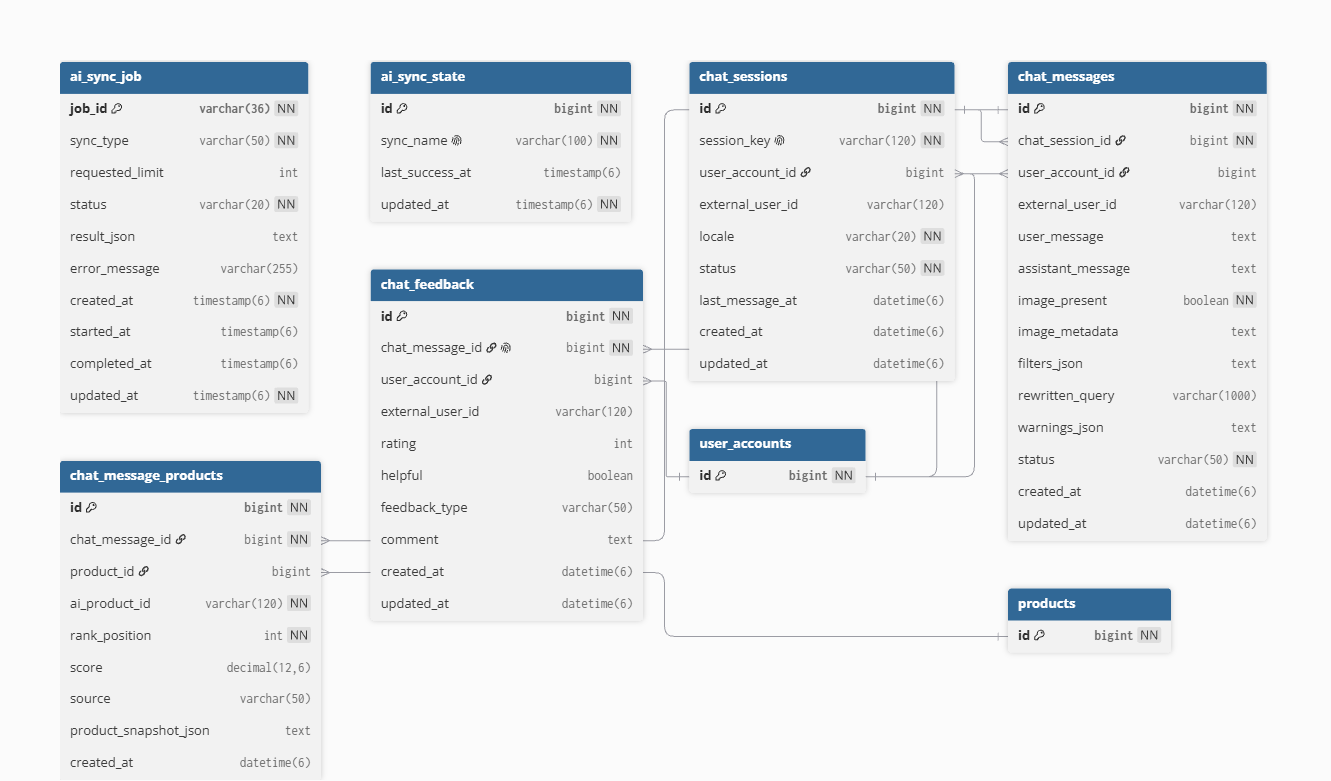
\includegraphics[
        width=\textwidth,
        height=0.72\textheight,
        keepaspectratio
    ]{Images/Thietkehethong/Tích hợp và đồng bộ AI.png}
    \caption{Sơ đồ dữ liệu tích hợp và đồng bộ AI}
    \label{fig:database-ai-integration}
\end{figure}

Theo Hình~\ref{fig:database-ai-integration}, một phiên hội thoại gồm nhiều tin
nhắn; mỗi tin nhắn có thể gắn với các sản phẩm được AI đề xuất và tối đa một phản
hồi đánh giá. Liên kết đến tài khoản và sản phẩm có thể rỗng để hỗ trợ khách chưa
đăng nhập cũng như bảo toàn bản chụp kết quả AI. Hai bảng
\texttt{ai\_sync\_job} và \texttt{ai\_sync\_state} không có khóa ngoại với
cụm hội thoại vì chúng theo dõi tiến trình lập chỉ mục ở cấp hệ thống, thay vì
biểu diễn một lượt tương tác của người dùng.

Bảng~\ref{tab:data-summary-ai-integration} tóm tắt chức năng của các bảng trong nhóm. Chỉ các bảng cốt lõi, đại diện trực tiếp cho luồng nghiệp vụ chính, được mô tả chi tiết trường dữ liệu.

\begin{longtable}{|>{\RaggedRight\arraybackslash}p{0.34\textwidth}|>{\RaggedRight\arraybackslash}p{0.56\textwidth}|}
    \caption{Các bảng thuộc nhóm tích hợp và đồng bộ AI}
    \label{tab:data-summary-ai-integration} \\
    \hline
    \textbf{Tên bảng} & \textbf{Chức năng} \\
    \hline
    \endfirsthead
    \multicolumn{2}{c}{\tablename\ \thetable\ (tiếp theo)} \\
    \hline
    \textbf{Tên bảng} & \textbf{Chức năng} \\
    \hline
    \endhead
    \texttt{ai\_sync\_job} & Công việc đồng bộ AI. \\
    \hline
    \texttt{ai\_sync\_state} & Trạng thái đồng bộ AI. \\
    \hline
    \texttt{chat\_sessions} & Phiên hội thoại. \\
    \hline
    \texttt{chat\_messages} & Tin nhắn hội thoại. \\
    \hline
    \texttt{chat\_message\_products} & Sản phẩm trong câu trả lời. \\
    \hline
    \texttt{chat\_feedback} & Phản hồi hội thoại. \\
    \hline
\end{longtable}

\paragraph{Các bảng cốt lõi.}

\begin{longtable}{|>{\RaggedRight\arraybackslash}p{0.25\textwidth}|>{\RaggedRight\arraybackslash}p{0.20\textwidth}|>{\RaggedRight\arraybackslash}p{0.45\textwidth}|}
    \caption{Mô tả chi tiết bảng \texttt{ai\_sync\_job} (Công việc đồng bộ AI)}
    \label{tab:data-dictionary-ai-sync-job} \\
    \hline
    \textbf{Tên trường} & \textbf{Kiểu dữ liệu} & \textbf{Mô tả} \\
    \hline
    \endfirsthead
    \multicolumn{3}{c}{\tablename\ \thetable\ (tiếp theo)} \\
    \hline
    \textbf{Tên trường} & \textbf{Kiểu dữ liệu} & \textbf{Mô tả} \\
    \hline
    \endhead
    \texttt{\seqsplit{job\_id}} & \texttt{varchar(36)} & Khóa chính. \\
        \hline
        \texttt{\seqsplit{sync\_type}} & \texttt{varchar(50)} & Loại tác vụ đồng bộ; bắt buộc. \\
        \hline
        \texttt{\seqsplit{requested\_limit}} & \texttt{int} & Số lượng bản ghi tối đa được yêu cầu xử lý. \\
        \hline
        \texttt{\seqsplit{status}} & \texttt{varchar(20)} & Trạng thái hiện tại; bắt buộc. \\
        \hline
        \texttt{\seqsplit{result\_json}} & \texttt{text} & Kết quả tác vụ ở định dạng JSON. \\
        \hline
        \texttt{\seqsplit{error\_message}} & \texttt{varchar(255)} & Thông báo lỗi khi xử lý. \\
        \hline
        \texttt{\seqsplit{created\_at}} & \texttt{timestamp(6)} & Thời điểm tạo bản ghi; bắt buộc. \\
        \hline
        \texttt{\seqsplit{started\_at}} & \texttt{timestamp(6)} & Thời điểm bắt đầu xử lý. \\
        \hline
        \texttt{\seqsplit{completed\_at}} & \texttt{timestamp(6)} & Thời điểm hoàn tất xử lý. \\
        \hline
        \texttt{\seqsplit{updated\_at}} & \texttt{timestamp(6)} & Thời điểm cập nhật gần nhất; bắt buộc. \\
        \hline
\end{longtable}

\begin{longtable}{|>{\RaggedRight\arraybackslash}p{0.25\textwidth}|>{\RaggedRight\arraybackslash}p{0.20\textwidth}|>{\RaggedRight\arraybackslash}p{0.45\textwidth}|}
    \caption{Mô tả chi tiết bảng \texttt{chat\_sessions} (Phiên hội thoại)}
    \label{tab:data-dictionary-chat-sessions} \\
    \hline
    \textbf{Tên trường} & \textbf{Kiểu dữ liệu} & \textbf{Mô tả} \\
    \hline
    \endfirsthead
    \multicolumn{3}{c}{\tablename\ \thetable\ (tiếp theo)} \\
    \hline
    \textbf{Tên trường} & \textbf{Kiểu dữ liệu} & \textbf{Mô tả} \\
    \hline
    \endhead
    \texttt{\seqsplit{id}} & \texttt{bigint} & Khóa chính tự tăng. \\
        \hline
        \texttt{\seqsplit{session\_key}} & \texttt{varchar(120)} & Khóa duy nhất của phiên hội thoại; bắt buộc; duy nhất. \\
        \hline
        \texttt{\seqsplit{user\_account\_id}} & \texttt{bigint} & Khóa ngoại tham chiếu \texttt{user\_accounts.id}. \\
        \hline
        \texttt{\seqsplit{external\_user\_id}} & \texttt{varchar(120)} & Định danh khách chưa đăng nhập. \\
        \hline
        \texttt{\seqsplit{locale}} & \texttt{varchar(20)} & Ngôn ngữ của phiên; bắt buộc. \\
        \hline
        \texttt{\seqsplit{status}} & \texttt{varchar(50)} & Trạng thái hiện tại; bắt buộc. \\
        \hline
        \texttt{\seqsplit{last\_message\_at}} & \texttt{datetime(6)} & Thời điểm có tin nhắn gần nhất. \\
        \hline
        \texttt{\seqsplit{created\_at}} & \texttt{datetime(6)} & Thời điểm tạo bản ghi. \\
        \hline
        \texttt{\seqsplit{updated\_at}} & \texttt{datetime(6)} & Thời điểm cập nhật gần nhất. \\
        \hline
\end{longtable}

\begin{longtable}{|>{\RaggedRight\arraybackslash}p{0.25\textwidth}|>{\RaggedRight\arraybackslash}p{0.20\textwidth}|>{\RaggedRight\arraybackslash}p{0.45\textwidth}|}
    \caption{Mô tả chi tiết bảng \texttt{chat\_messages} (Tin nhắn hội thoại)}
    \label{tab:data-dictionary-chat-messages} \\
    \hline
    \textbf{Tên trường} & \textbf{Kiểu dữ liệu} & \textbf{Mô tả} \\
    \hline
    \endfirsthead
    \multicolumn{3}{c}{\tablename\ \thetable\ (tiếp theo)} \\
    \hline
    \textbf{Tên trường} & \textbf{Kiểu dữ liệu} & \textbf{Mô tả} \\
    \hline
    \endhead
    \texttt{\seqsplit{id}} & \texttt{bigint} & Khóa chính tự tăng. \\
        \hline
        \texttt{\seqsplit{chat\_session\_id}} & \texttt{bigint} & Khóa ngoại tham chiếu \texttt{chat\_sessions.id}; bắt buộc. \\
        \hline
        \texttt{\seqsplit{user\_account\_id}} & \texttt{bigint} & Khóa ngoại tham chiếu \texttt{user\_accounts.id}. \\
        \hline
        \texttt{\seqsplit{external\_user\_id}} & \texttt{varchar(120)} & Định danh khách chưa đăng nhập. \\
        \hline
        \texttt{\seqsplit{user\_message}} & \texttt{text} & Nội dung người dùng gửi. \\
        \hline
        \texttt{\seqsplit{assistant\_message}} & \texttt{text} & Nội dung trợ lý trả lời. \\
        \hline
        \texttt{\seqsplit{image\_present}} & \texttt{boolean} & Cho biết yêu cầu có kèm hình ảnh; bắt buộc. \\
        \hline
        \texttt{\seqsplit{image\_metadata}} & \texttt{text} & Siêu dữ liệu của hình ảnh. \\
        \hline
        \texttt{\seqsplit{filters\_json}} & \texttt{text} & Bộ lọc tìm kiếm ở định dạng JSON. \\
        \hline
        \texttt{\seqsplit{rewritten\_query}} & \texttt{varchar(1000)} & Truy vấn đã được AI viết lại. \\
        \hline
        \texttt{\seqsplit{warnings\_json}} & \texttt{text} & Danh sách cảnh báo ở định dạng JSON. \\
        \hline
        \texttt{\seqsplit{status}} & \texttt{varchar(50)} & Trạng thái hiện tại; bắt buộc. \\
        \hline
        \texttt{\seqsplit{created\_at}} & \texttt{datetime(6)} & Thời điểm tạo bản ghi. \\
        \hline
        \texttt{\seqsplit{updated\_at}} & \texttt{datetime(6)} & Thời điểm cập nhật gần nhất. \\
        \hline
\end{longtable}



\subsubsection{Thiết kế chỉ mục và đồng bộ dữ liệu MySQL--Qdrant}

MySQL là nguồn dữ liệu chuẩn, còn Qdrant chỉ lưu dữ liệu dẫn xuất phục vụ truy hồi. Mỗi điểm trong chỉ mục sử dụng \texttt{product\_id} làm khóa liên kết ổn định với sản phẩm trong MySQL. Vector văn bản và vector hình ảnh có thể được tổ chức trong các collection riêng do khác nhau về mô hình embedding, số chiều và chiến lược truy vấn. Payload chỉ chứa metadata cần thiết cho lọc và xếp hạng, chẳng hạn danh mục, thuộc tính, khoảng giá, trạng thái khả dụng và thời điểm cập nhật.

Giá, tồn kho và trạng thái trong payload là ảnh chụp tại thời điểm lập chỉ mục nên có thể chậm hơn dữ liệu nghiệp vụ. Vì vậy, Qdrant chỉ được dùng để tìm tập ứng viên; Spring Boot luôn nạp lại sản phẩm từ MySQL, loại các bản ghi không còn hợp lệ và sử dụng giá cùng tồn kho hiện hành trước khi trả kết quả cho Frontend.

Hệ thống hỗ trợ đồng bộ toàn bộ, đồng bộ tăng dần, đồng bộ một sản phẩm và xóa sản phẩm khỏi chỉ mục. Spring Boot tạo DTO lập chỉ mục từ dữ liệu MySQL; AI Service tạo embedding, xây dựng payload rồi thực hiện upsert hoặc delete trong Qdrant. Các thao tác dùng \texttt{product\_id} ổn định nên có thể thực hiện lại an toàn khi gặp lỗi tạm thời.

\begin{figure}[H]
    \centering
    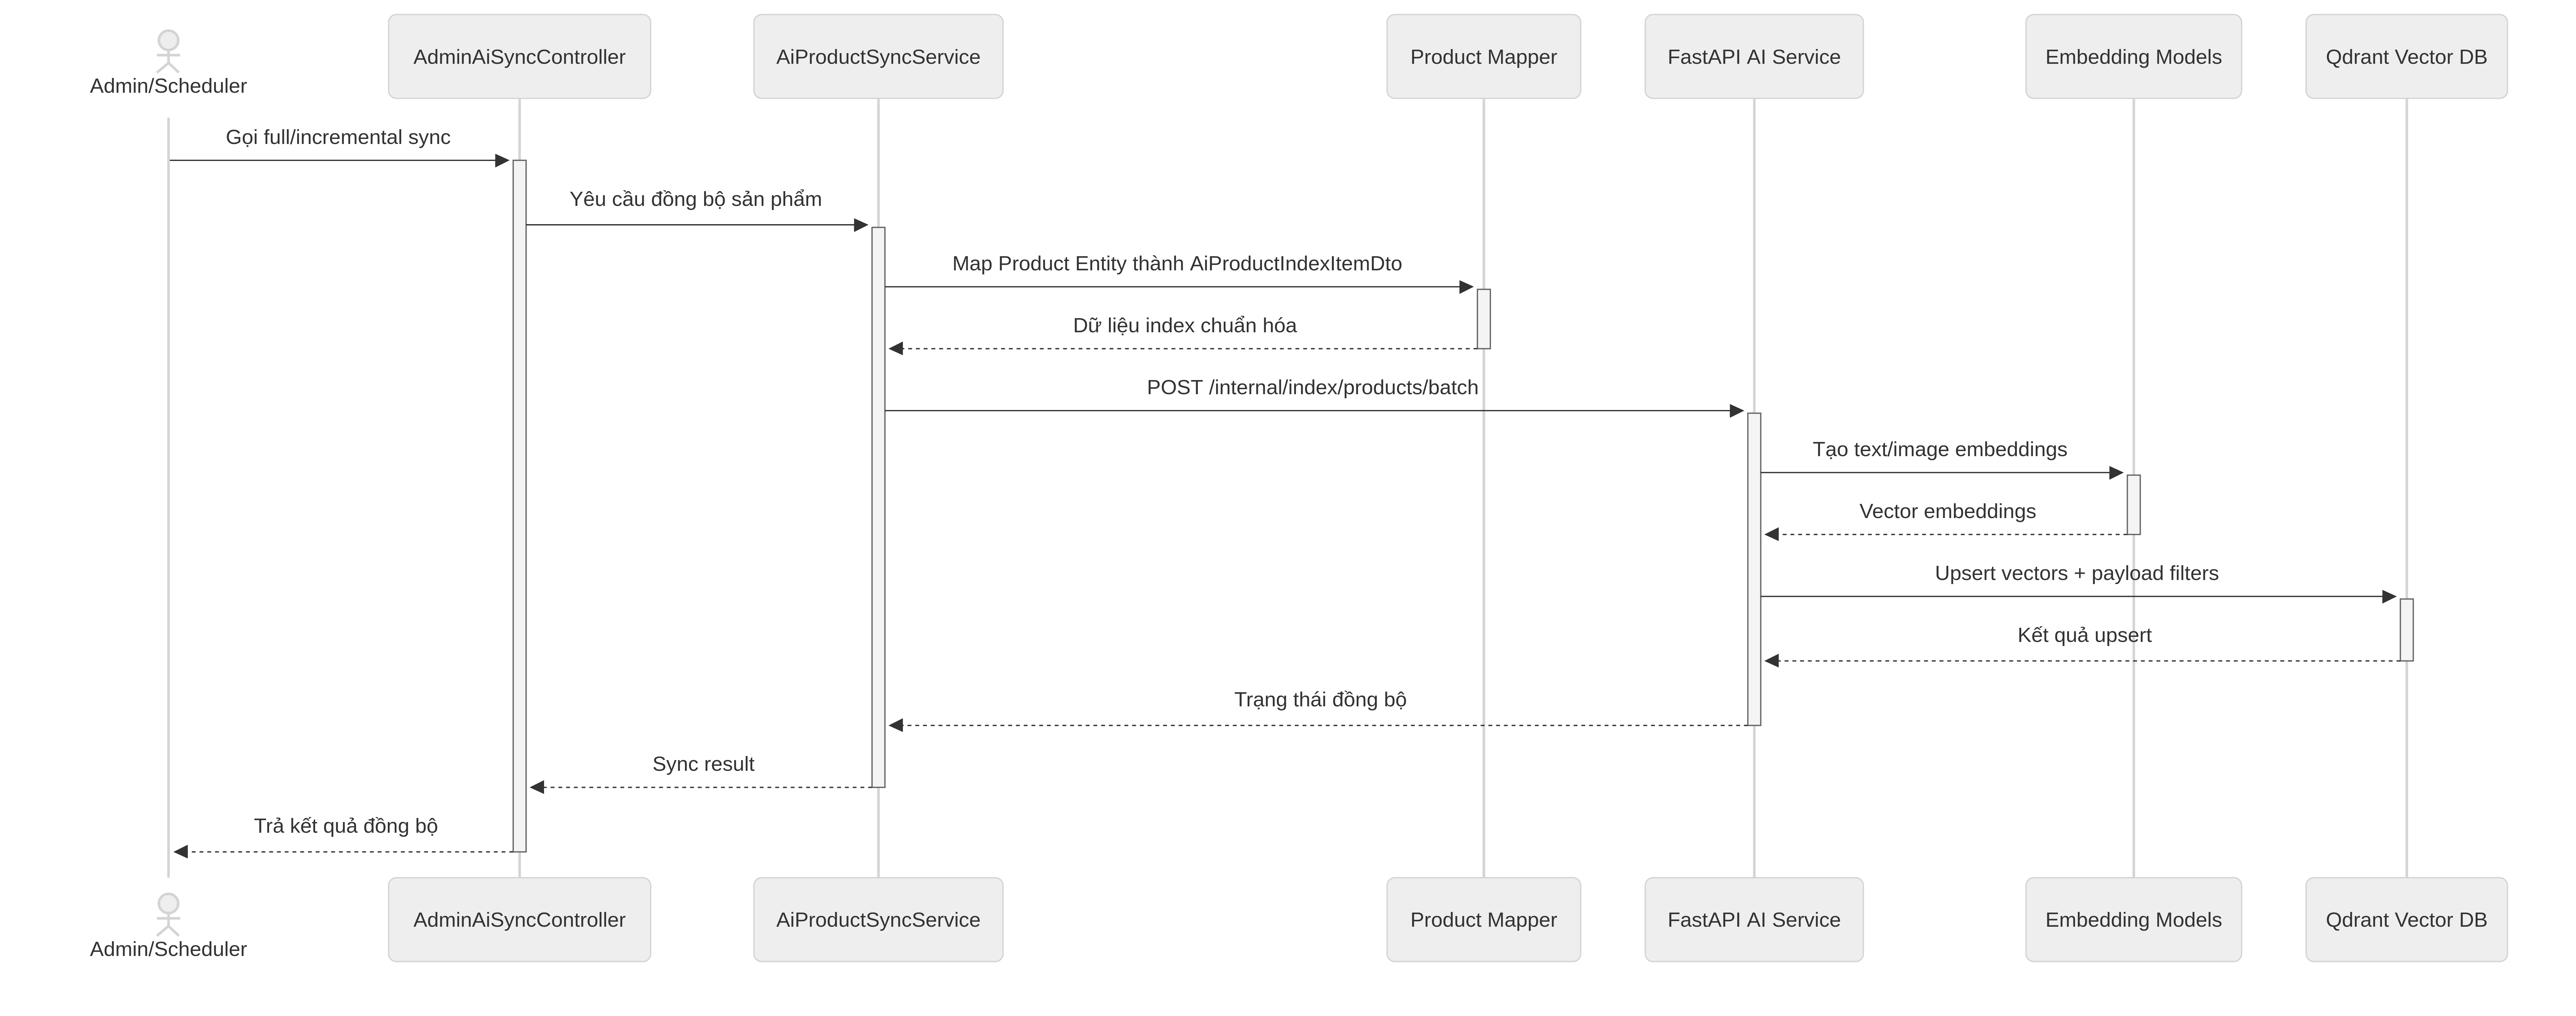
\includegraphics[width=0.95\textwidth]{Images/Thietkehethong/dongboAI.png}
    \caption{Luồng đồng bộ dữ liệu từ MySQL sang Qdrant}
    \label{fig:ai-sync-flow}
\end{figure}

Tiến trình được ghi nhận trong \texttt{ai\_sync\_job}, còn \texttt{ai\_sync\_state} lưu mốc đồng bộ thành công gần nhất. Một công việc có thể hoàn thành toàn bộ, thất bại hoặc thành công một phần; kết quả cần ghi số bản ghi thành công, số bản ghi lỗi và các mã sản phẩm cần thử lại. Lỗi cập nhật Qdrant không hoàn tác giao dịch nghiệp vụ trong MySQL vì chỉ mục có thể được tái tạo.

\subsection{Thiết kế các chức năng chính}

Các activity diagram của các luồng chính đã được trình bày tại Chương 5. Phần này không lặp lại luồng điều khiển giữa các tác nhân mà tập trung vào quyết định thiết kế bên trong: quy tắc kiểm tra, ranh giới transaction, chuyển trạng thái, dữ liệu đầu ra và phương án suy giảm khi một phụ thuộc không khả dụng.

\subsubsection{Checkout và quản lý vòng đời đơn hàng}

Hai thao tác preview và confirm được tách riêng. Preview là phép đọc để tính giá dự kiến, giảm giá tự động và coupon; thao tác này không tạo đơn hay giữ tồn kho. Confirm thực hiện lại toàn bộ kiểm tra trong transaction: giỏ và địa chỉ thuộc người dùng, sản phẩm còn bán, biến thể đủ số lượng, giá còn hiệu lực và coupon còn áp dụng.

Khi các điều kiện hợp lệ, Backend tạo \texttt{Order}, chụp lại địa chỉ và thông tin từng dòng hàng, áp dụng coupon, giữ tồn kho, tạo lịch sử trạng thái rồi chuyển giỏ sang \texttt{CHECKED\_OUT}. Bất kỳ lỗi nào trong chuỗi ghi bắt buộc đều làm rollback transaction. Luồng đặt hàng COD được thể hiện tại Hình~\ref{fig:activity-cod-checkout}; phần xác nhận và cập nhật trạng thái COD được thể hiện tại Hình~\ref{fig:activity-cod-confirmation}.

Trạng thái đơn hàng được quản lý bằng một tập chuyển tiếp hữu hạn. Mỗi lệnh phải kiểm tra trạng thái nguồn, vai trò người thực hiện và tác động kèm theo đối với tồn kho hoặc thanh toán. Lịch sử trạng thái được ghi bất biến để truy vết; không cập nhật trực tiếp trạng thái đơn mà bỏ qua service nghiệp vụ.

\begin{figure}[H]
    \centering
    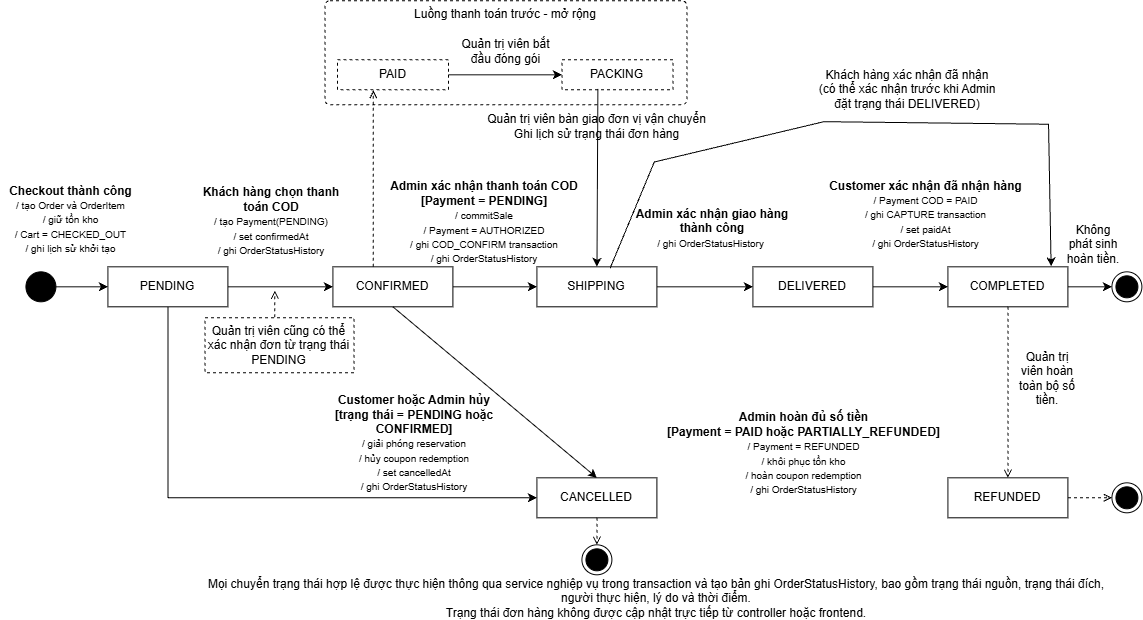
\includegraphics[width=0.98\textwidth]{Images/Thietkehethong/Thiết kế vòng đời trạng thái đơn hàng và các tác động nghiệp vụ.drawio.png}
    \caption{Thiết kế vòng đời trạng thái đơn hàng và các tác động nghiệp vụ}
    \label{fig:order-state-design}
\end{figure}

Hình~\ref{fig:order-state-design} phân biệt luồng COD đang được sử dụng với nhánh thanh toán trước dự kiến mở rộng. Trong luồng COD, đơn được tạo ở trạng thái \texttt{PENDING}, chuyển sang \texttt{CONFIRMED} sau khi phương thức thanh toán được xác lập, rồi sang \texttt{SHIPPING} khi quản trị viên xác nhận khoản COD và bàn giao vận chuyển. Quản trị viên có thể đánh dấu giao hàng thành công để chuyển đơn sang \texttt{DELIVERED}; khách hàng xác nhận đã nhận hàng từ \texttt{SHIPPING} hoặc \texttt{DELIVERED} để hoàn tất đơn. Tại thời điểm đó, khoản COD được ghi nhận là đã thanh toán và transaction thu tiền được lưu để đối soát.

Đơn chỉ được hủy từ \texttt{PENDING} hoặc \texttt{CONFIRMED}. Thao tác hủy giải phóng phần tồn kho đã giữ, hoàn lượt sử dụng coupon và ghi lịch sử chuyển trạng thái. Đối với đơn đã hoàn thành, hoàn đủ số tiền chuyển đơn sang \texttt{REFUNDED}, đồng thời khôi phục tồn kho và coupon theo transaction hoàn tiền. Nhánh \texttt{PAID}--\texttt{PACKING} được biểu diễn bằng nét đứt để thể hiện khả năng tích hợp thanh toán trước mà không làm thay đổi luồng COD hiện hành. Mọi chuyển tiếp hợp lệ đều đi qua service nghiệp vụ trong transaction và sinh bản ghi \texttt{OrderStatusHistory}; controller không được cập nhật trực tiếp trạng thái đơn hàng.

\subsubsection{Tìm kiếm sản phẩm bằng AI}

Luồng tương tác đa phương thức đã được mô tả tại Hình~\ref{fig:activity-multimodal-search}. Về thiết kế xử lý, request được quy về một mô hình chung gồm truy vấn văn bản tùy chọn, ảnh tùy chọn, vùng quan tâm, bộ lọc và giới hạn kết quả. Endpoint \texttt{auto} lựa chọn nhánh phù hợp theo dữ liệu thực nhận; endpoint chuyên biệt từ chối request thiếu đầu vào bắt buộc.

Pipeline gồm bốn giai đoạn. Thứ nhất, Query Understanding chuẩn hóa truy vấn và sinh bộ lọc có cấu trúc. Thứ hai, ảnh được kiểm tra và cắt theo vùng người dùng chọn hoặc vùng YOLO phát hiện; YOLO không phải phụ thuộc bắt buộc. Thứ ba, embedding provider tạo vector cùng không gian với collection Qdrant. Cuối cùng, Search Service truy hồi tập ứng viên, áp dụng filter và tùy chọn reranking.

Kết quả AI chỉ chứa \texttt{product\_id}, điểm số, nguồn truy hồi và cảnh báo. \texttt{ProductCardResolver} tại Spring Boot nạp lại dữ liệu hiện hành từ MySQL, loại ứng viên không hợp lệ và bảo toàn thứ tự còn lại. Khi AI Service lỗi và request có truy vấn văn bản, Backend có thể dùng keyword fallback; nếu chỉ có ảnh, hệ thống trả trạng thái suy giảm rõ ràng thay vì tạo kết quả không có căn cứ.

\begin{figure}[H]
    \centering
    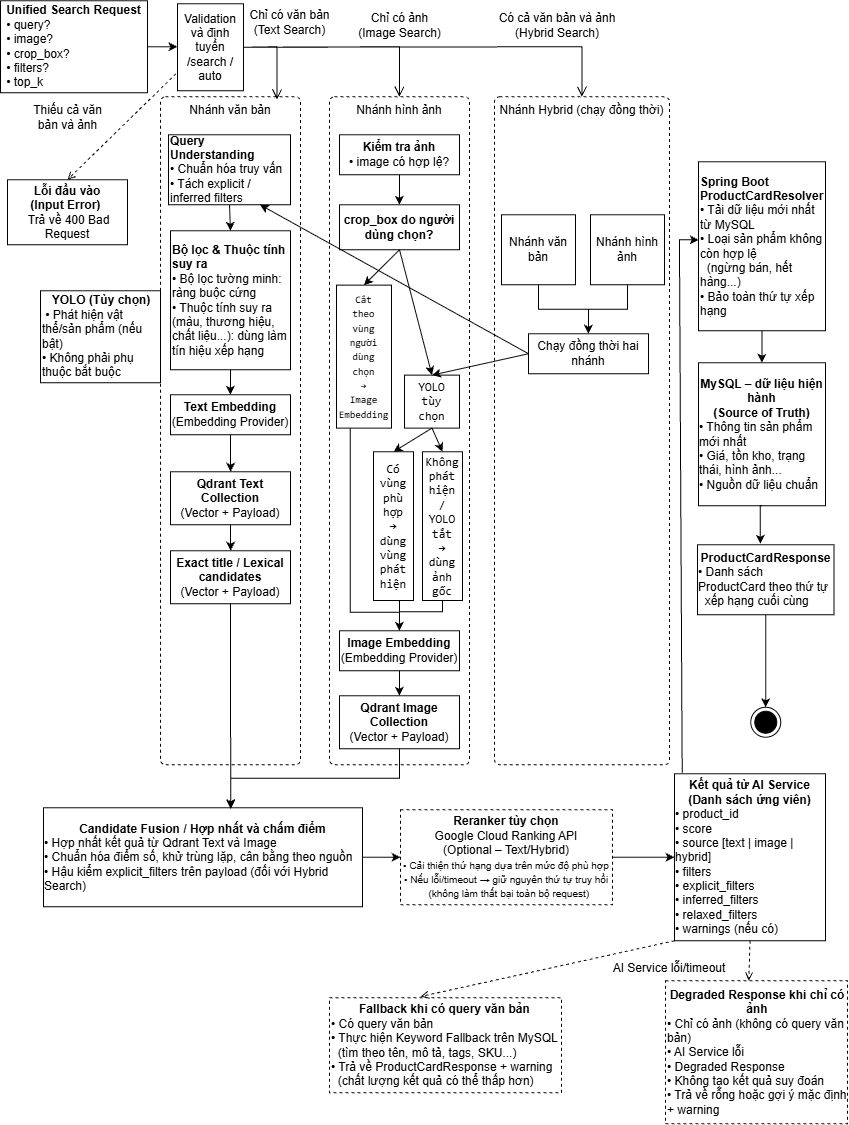
\includegraphics[width=0.92\textwidth,height=0.78\textheight,keepaspectratio]{Images/Thietkehethong/Pipeline xử lý tìm kiếm sản phẩm đa phương thức.drawio.png}
    \caption{Pipeline xử lý tìm kiếm sản phẩm đa phương thức}
    \label{fig:ai-search-pipeline}
\end{figure}

Hình~\ref{fig:ai-search-pipeline} mô tả cách endpoint \texttt{/search/auto} kiểm tra request và định tuyến theo dữ liệu đầu vào. Với truy vấn văn bản, Query Understanding chuẩn hóa câu truy vấn, phân biệt bộ lọc tường minh với thuộc tính suy ra và tạo text embedding. Tập ứng viên vector từ Qdrant được kết hợp với ứng viên khớp tên hoặc lexical khi chức năng này được bật. Với truy vấn ảnh, vùng \texttt{crop\_box} do người dùng chọn được ưu tiên và đưa thẳng đến bước embedding; nếu không có vùng chọn, hệ thống có thể dùng YOLO để phát hiện đối tượng, đồng thời quay về ảnh gốc khi YOLO bị tắt hoặc không tìm được vùng phù hợp.

Tìm kiếm kết hợp thực thi đồng thời nhánh văn bản và nhánh ảnh, sau đó hợp nhất ứng viên, khử trùng lặp, cân bằng điểm theo nguồn và hậu kiểm các ràng buộc tường minh trên payload. Reranker là bước tùy chọn cho tìm kiếm văn bản và kết hợp; lỗi hoặc timeout tại bước này không làm mất kết quả truy hồi ban đầu. AI Service chỉ trả định danh sản phẩm, điểm số, nguồn và thông tin bộ lọc. Spring Boot dùng \texttt{ProductCardResolver} để nạp dữ liệu hiện hành từ MySQL, loại sản phẩm không còn hợp lệ và bảo toàn thứ tự xếp hạng trước khi tạo \texttt{ProductCardResponse}. Khi AI Service không khả dụng, request có văn bản được chuyển sang keyword fallback trên MySQL; request chỉ có ảnh nhận response suy giảm rõ ràng thay vì kết quả suy đoán.

\subsubsection{Trợ lý hội thoại}

\begin{figure}[H]
    \centering
    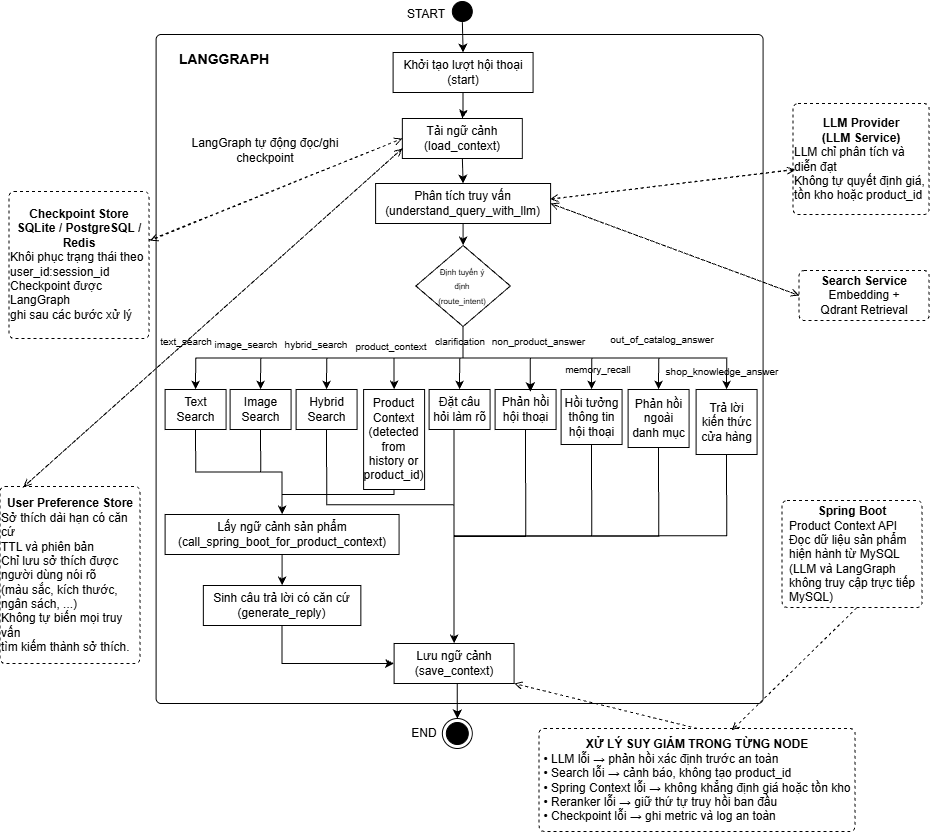
\includegraphics[width=0.96\textwidth,height=0.80\textheight,keepaspectratio]{Images/Thietkehethong/Thiết kế đồ thị trạng thái của trợ lý hội thoại.drawio.png}
    \caption{Thiết kế đồ thị trạng thái của trợ lý hội thoại}
    \label{fig:assistant-state-graph}
\end{figure}

Luồng tương tác giữa người dùng, Backend và AI Service đã được trình bày tại Hình~\ref{fig:activity-multiturn-chat}. Hình~\ref{fig:assistant-state-graph} tập trung vào cách AI Service điều phối một lượt hội thoại bằng đồ thị trạng thái LangGraph. Trạng thái dùng chung mang định danh phiên, lịch sử hội thoại đã rút gọn, sở thích người dùng có căn cứ, kết quả phân tích truy vấn, tập ứng viên sản phẩm và các cảnh báo phát sinh. Cách tổ chức này cho phép từng nút chỉ đọc và cập nhật phần dữ liệu cần thiết, đồng thời duy trì ngữ cảnh nhất quán giữa các lượt trao đổi.

Mỗi lượt xử lý bắt đầu tại nút \texttt{start}, sau đó \texttt{load\_context} nạp checkpoint và thông tin sở thích liên quan. Nút \texttt{understand\_query\_with\_llm} phân tích nội dung đầu vào; \texttt{route\_intent} sử dụng kết quả này để chọn nhánh xử lý. Truy vấn sản phẩm được định tuyến đến tìm kiếm văn bản, tìm kiếm ảnh hoặc tìm kiếm kết hợp. Kết quả tìm kiếm chỉ chứa tập ứng viên và được chuyển đến \texttt{call\_spring\_boot\_for\_product\_context} để lấy dữ liệu sản phẩm hiện hành trước khi \texttt{generate\_reply} sinh câu trả lời. Nếu truy vấn đã chứa đủ tham chiếu đến sản phẩm trong ngữ cảnh hội thoại, workflow có thể đi thẳng đến bước lấy ngữ cảnh sản phẩm mà không thực hiện một lượt tìm kiếm mới.

Các ý định không yêu cầu truy hồi sản phẩm được tách thành những nhánh riêng: đặt câu hỏi làm rõ, phản hồi hội thoại thông thường, hồi tưởng thông tin đã được ghi nhận, phản hồi truy vấn ngoài danh mục và trả lời kiến thức cửa hàng. Việc tách nhánh giúp áp dụng chỉ dẫn và giới hạn dữ liệu phù hợp cho từng loại câu trả lời, thay vì sử dụng một prompt chung cho mọi tình huống. Dù đi qua nhánh nào, kết quả cuối cùng đều hội tụ tại \texttt{save\_context} trước khi kết thúc lượt xử lý, nhờ đó trạng thái mới có thể được dùng cho câu hỏi tiếp theo.

Các khối nằm ngoài biên LangGraph thể hiện phụ thuộc tích hợp, không phải trạng thái nghiệp vụ. LLM Provider hỗ trợ phân tích truy vấn và sinh ngôn ngữ; Search Service thực hiện truy hồi ứng viên; Spring Boot Product Context API cung cấp dữ liệu chuẩn về sản phẩm. Checkpoint Store lưu trạng thái thực thi theo phiên, trong khi User Preference Store chỉ lưu những sở thích đủ căn cứ để tái sử dụng. Trợ lý không truy cập trực tiếp MySQL và không xem dữ liệu trong chỉ mục tìm kiếm là nguồn sự thật cuối cùng.

Thiết kế cũng quy định cơ chế suy giảm tại từng điểm phụ thuộc. Khi reranker gặp lỗi, hệ thống giữ thứ tự truy hồi ban đầu; khi Search Service không khả dụng, workflow không tự tạo định danh sản phẩm; và khi không lấy được ngữ cảnh từ Spring Boot, câu trả lời không khẳng định giá hoặc tồn kho. Lỗi mô hình được chuyển thành phản hồi an toàn, còn lỗi checkpoint được ghi nhận qua log và metric để phục vụ giám sát. Nhờ vậy, sự cố của một thành phần AI không làm phát sinh thông tin giao dịch không có căn cứ.

\subsection{Thiết kế giao tiếp và tích hợp}

\subsubsection{Hợp đồng giao tiếp giữa các dịch vụ}

Frontend chỉ gọi API công khai của Spring Boot. Backend tiếp nhận danh tính người dùng, kiểm tra quyền và điều phối nghiệp vụ trước khi gọi AI Service qua API nội bộ. AI Service có thể đọc ngữ cảnh giới hạn từ Spring Boot nhưng không truy cập trực tiếp MySQL. API quản trị dùng tiền tố \texttt{/admin}, còn endpoint tích hợp giữa hai dịch vụ dùng \texttt{/internal}.

Request và response thông thường sử dụng JSON; dữ liệu ảnh tuân theo hợp đồng của endpoint tìm kiếm tương ứng. DTO xác định rõ trường bắt buộc, giới hạn dữ liệu và cấu trúc lồng nhau. Spring Boot không truyền JPA Entity sang AI Service mà chuyển sản phẩm thành indexing DTO dạng \texttt{snake\_case}.

Luồng lập chỉ mục được khởi tạo qua các API quản trị \texttt{POST} \path{/admin/ai-sync/full}, \path{/admin/ai-sync/incremental} và \path{/admin/ai-sync/products/\{productId\}}. Tại ranh giới nội bộ, AI Service cung cấp \texttt{POST} \path{/internal/index/products/batch}, \texttt{POST} \path{/internal/index/products/\{product_id\}} và \texttt{DELETE} \path{/internal/index/products/\{product_id\}}. Các endpoint ghi chỉ mục sử dụng định danh sản phẩm ổn định để hỗ trợ gọi lại an toàn.

Indexing DTO chứa định danh, nội dung mô tả, phân loại, thuộc tính biến thể, giá hiệu lực, tổng tồn, trạng thái khả dụng, URL ảnh và thời điểm cập nhật. \texttt{product\_id} là khóa liên kết ổn định giữa MySQL và Qdrant.

AI Service dùng DTO để tạo nội dung embedding và payload Qdrant nhưng không trả payload đó trực tiếp cho Frontend. Search response chỉ cần định danh ứng viên, điểm số, nguồn truy hồi, bộ lọc đã áp dụng và cảnh báo. Assistant response bổ sung nội dung trả lời, mã phiên và danh sách định danh sản phẩm có căn cứ.

\begin{table}[H]
    \centering
    \caption{Các hợp đồng chính giữa Spring Boot và AI Service}
    \label{tab:spring-ai-contracts}
    \begin{tabularx}{\textwidth}{|p{0.20\textwidth}|p{0.30\textwidth}|X|}
        \hline
        \textbf{Hợp đồng} & \textbf{Dữ liệu chính} & \textbf{Ràng buộc thiết kế} \\
        \hline
        Index product & Product ID, text fields, attributes, price, stock, images, updated time & Upsert theo Product ID; không phụ thuộc cấu trúc JPA Entity. \\
        \hline
        Search request & Modality, query/image, ROI, filters, top-k & Giới hạn kích thước; loại bỏ filter không hợp lệ trước khi truy hồi. \\
        \hline
        Search response & Candidate ID, score, source, warnings & Không dùng làm dữ liệu giá hoặc tồn kho cuối cùng. \\
        \hline
        Assistant request & Session ID, user key, message, context tối thiểu & Không truyền token người dùng hoặc dữ liệu cá nhân không cần thiết. \\
        \hline
        Assistant response & Answer, candidate IDs, warnings, trace metadata an toàn & Candidate phải được resolve lại; metadata nội bộ không trả ra giao diện. \\
        \hline
    \end{tabularx}
\end{table}

\subsubsection{Xác thực và xử lý lỗi tích hợp}

Request người dùng được xác thực bằng JWT; quyền quản trị và quyền sở hữu tài nguyên được kiểm tra tại Spring Boot. Kết nối nội bộ sử dụng header \texttt{X-Internal-API-Key}; khóa này không được gửi cho Frontend hoặc ghi vào log. MySQL, Qdrant và endpoint nội bộ chỉ được truy cập trong phạm vi mạng được phép.

Integration client cấu hình connection timeout, read timeout và correlation ID. Response lỗi có mã ổn định và thông điệp an toàn; chi tiết kỹ thuật chỉ được ghi trong log đã loại dữ liệu nhạy cảm. Spring Boot và AI Service cùng kiểm tra schema, giới hạn kích thước ảnh, tọa độ ROI, top-k và filter trước khi xử lý.

Retry chỉ áp dụng cho lỗi tạm thời và thao tác có tính lặp. Search có thể retry giới hạn; indexing upsert có thể gọi lại nhờ \texttt{product\_id} ổn định. Checkout và cập nhật trạng thái đơn không được retry tự động nếu chưa có idempotency key. Khi AI Service không khả dụng, tìm kiếm văn bản chuyển sang keyword fallback; các nghiệp vụ thương mại điện tử cốt lõi vẫn hoạt động.

\subsection*{Kết chương}

Chương này đã xác định thiết kế hệ thống từ kiến trúc tổng thể đến dữ liệu, các chức năng trọng tâm và hợp đồng tích hợp. Các quyết định nhất quán xuyên suốt gồm Spring Boot kiểm soát nghiệp vụ và API công khai, MySQL là nguồn dữ liệu chuẩn, AI Service có thể suy giảm độc lập và Qdrant là chỉ mục có thể tái tạo. Các activity diagram được trình bày ở Chương 5; Chương 6 bổ sung sơ đồ trạng thái đơn hàng, pipeline tìm kiếm và đồ thị workflow của trợ lý để làm rõ các quyết định thiết kế bên trong.
